\chapter{Adria International Raceway results}
\label{app:Adria}
%
In this appendix are reported the main results of the simulation in the Adria circuit for each model considered.
%
\section{Slip Control Adherence Ellipse Constraint}
%
\begin{figure}[!h]
    \centering
    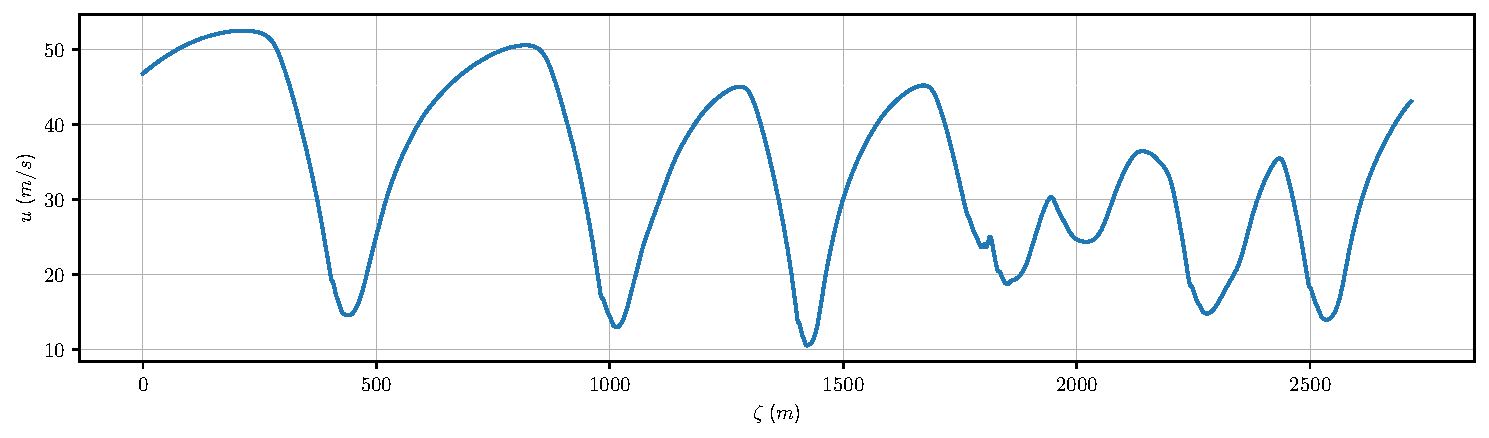
\includegraphics[width=\linewidth]{Circuit/u_P_SCell.pdf}
    \caption{Longitudinal speed}
    \label{fig:uSCE}
\end{figure}
%
\begin{figure}[!h]
    \centering
    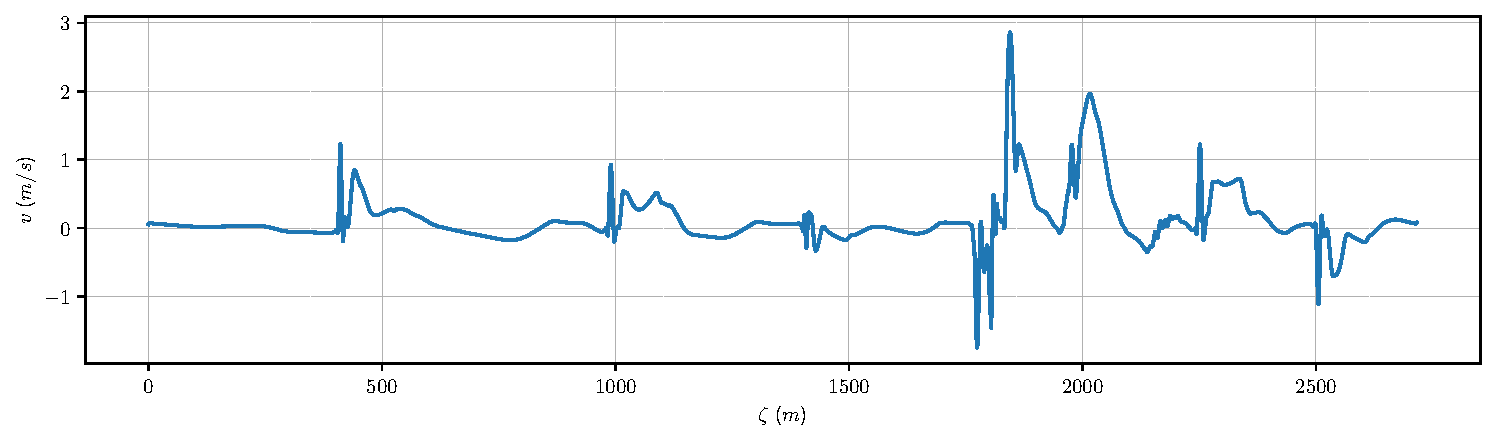
\includegraphics[width=\linewidth]{Circuit/v_P_SCell.pdf}
    \caption{Lateral speed}
    \label{fig:vSCE}
\end{figure}
%
\begin{figure}[!h]
    \centering
    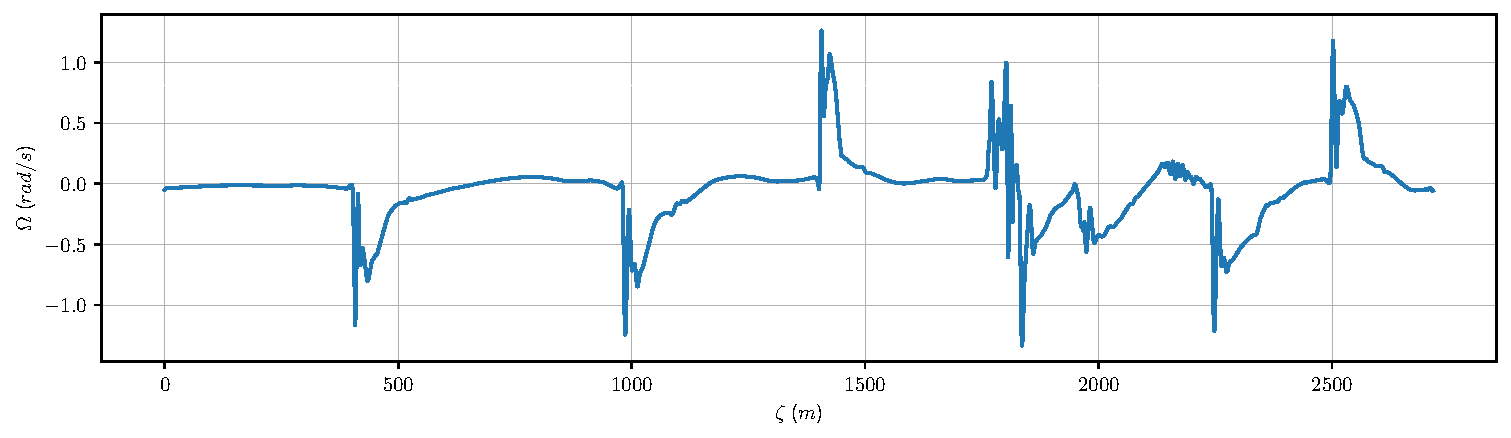
\includegraphics[width=\linewidth]{Circuit/Omega_P_SCell.pdf}
    \caption{Yaw rate}
    \label{fig:OmegaSCE}
\end{figure}
%
\begin{figure}[!h]
    \centering
    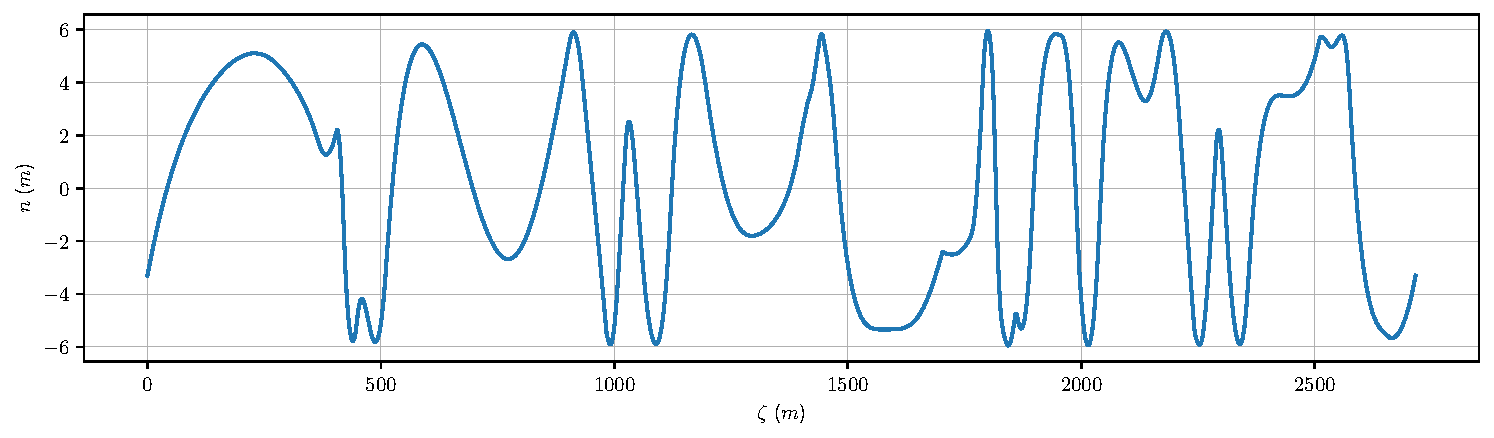
\includegraphics[width=\linewidth]{Circuit/n_P_SCell.pdf}
    \caption{Centreline deviation}
    \label{fig:nSCE}
\end{figure}
%
\begin{figure}[!h]
    \centering
    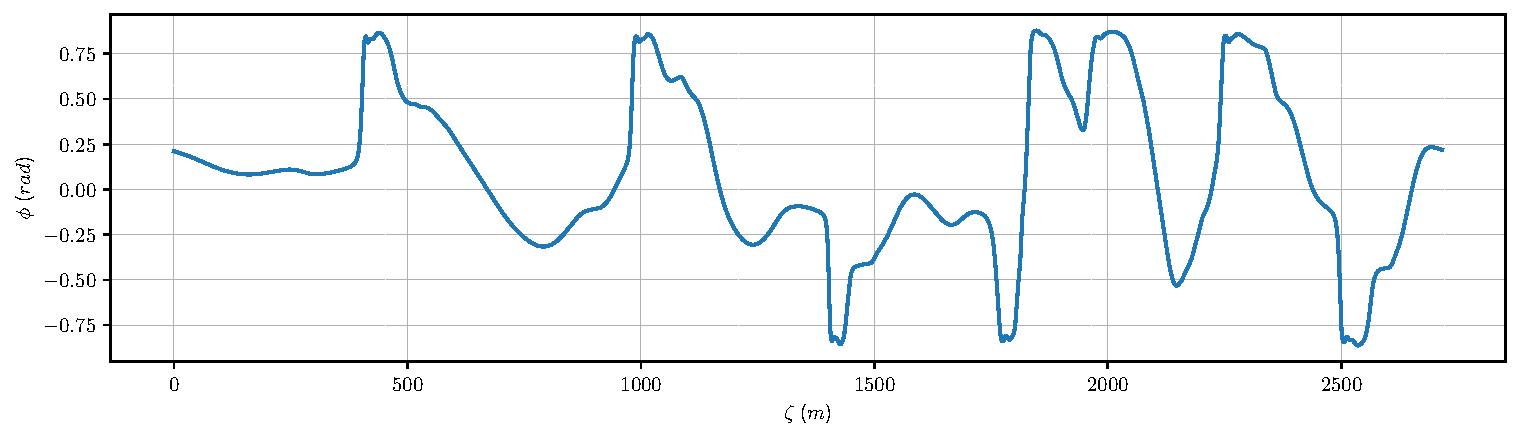
\includegraphics[width=\linewidth]{Circuit/phi_P_SCell.pdf}
    \caption{Roll angle}
    \label{fig:phiSCE}
\end{figure}
%
\begin{figure}[!h]
    \centering
    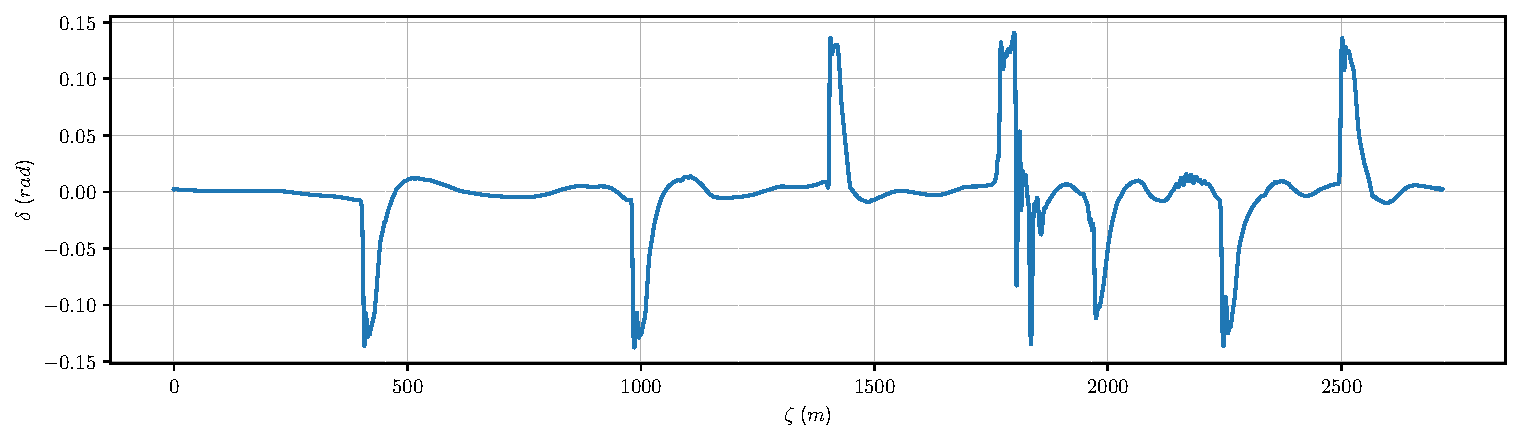
\includegraphics[width=\linewidth]{Circuit/delta_P_SCell.pdf}
    \caption{Steer angle}
    \label{fig:deltaSCE}
\end{figure}
%
\begin{figure}[!h]
    \centering
    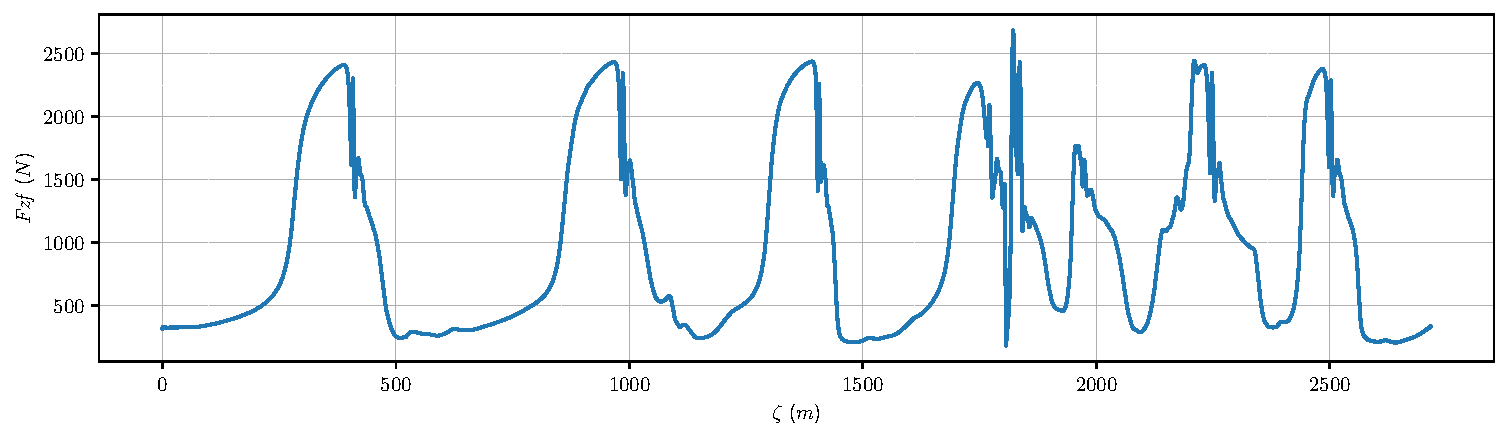
\includegraphics[width=\linewidth]{Circuit/Fzf_P_SCell.pdf}
    \caption{Vertical load front}
    \label{fig:FZFSCE}
\end{figure}
%
\begin{figure}[!h]
    \centering
    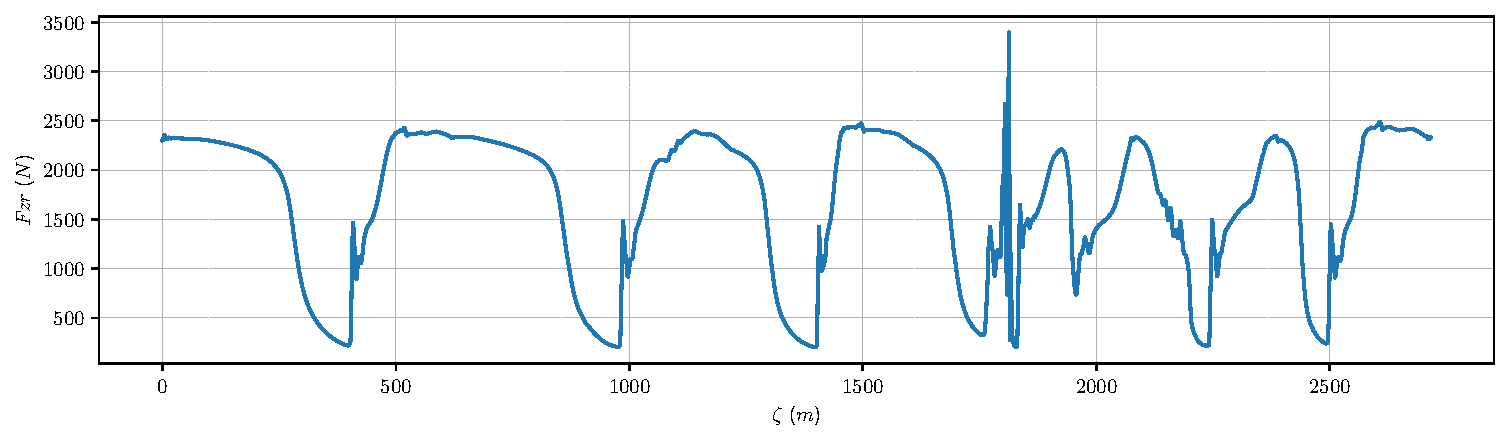
\includegraphics[width=\linewidth]{Circuit/Fzr_P_SCell.pdf}
    \caption{Vertical load rear}
    \label{fig:FZFSCE}
\end{figure}
%
\begin{figure}[!h]
    \begin{subfigure}{0.5\linewidth}
        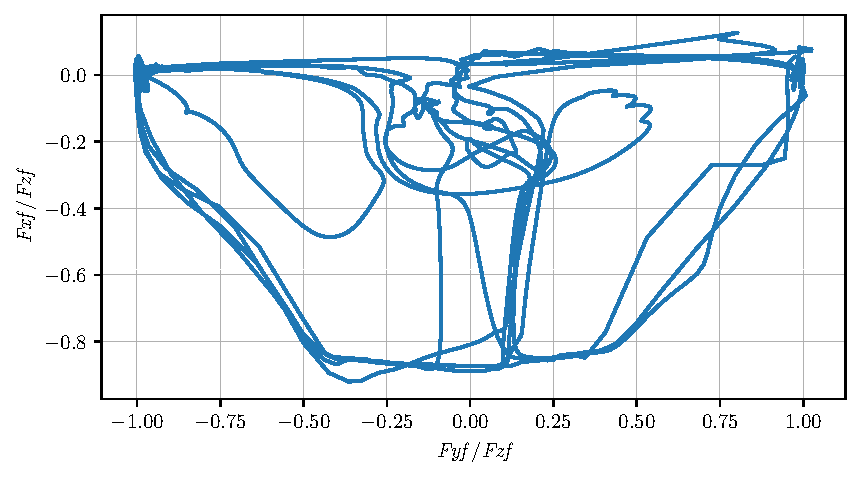
\includegraphics[width=\linewidth]{Circuit/EFront_P_SCell.pdf}
        \caption{Front}
        \label{fig:FESCE}
    \end{subfigure}%
    \begin{subfigure}{0.5\linewidth}
        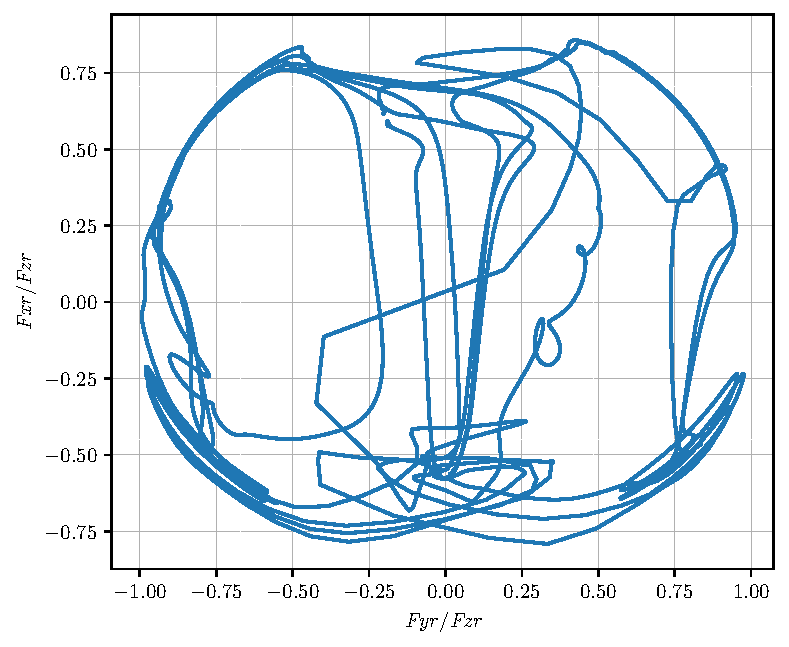
\includegraphics[width=\linewidth]{Circuit/ERear_P_SCell.pdf}
        \caption{Rear}
        \label{fig:RESCE}
    \end{subfigure}
    \caption{Ellipse of adherence}
\end{figure}
%
%
\begin{figure}[!h]
    \centering
    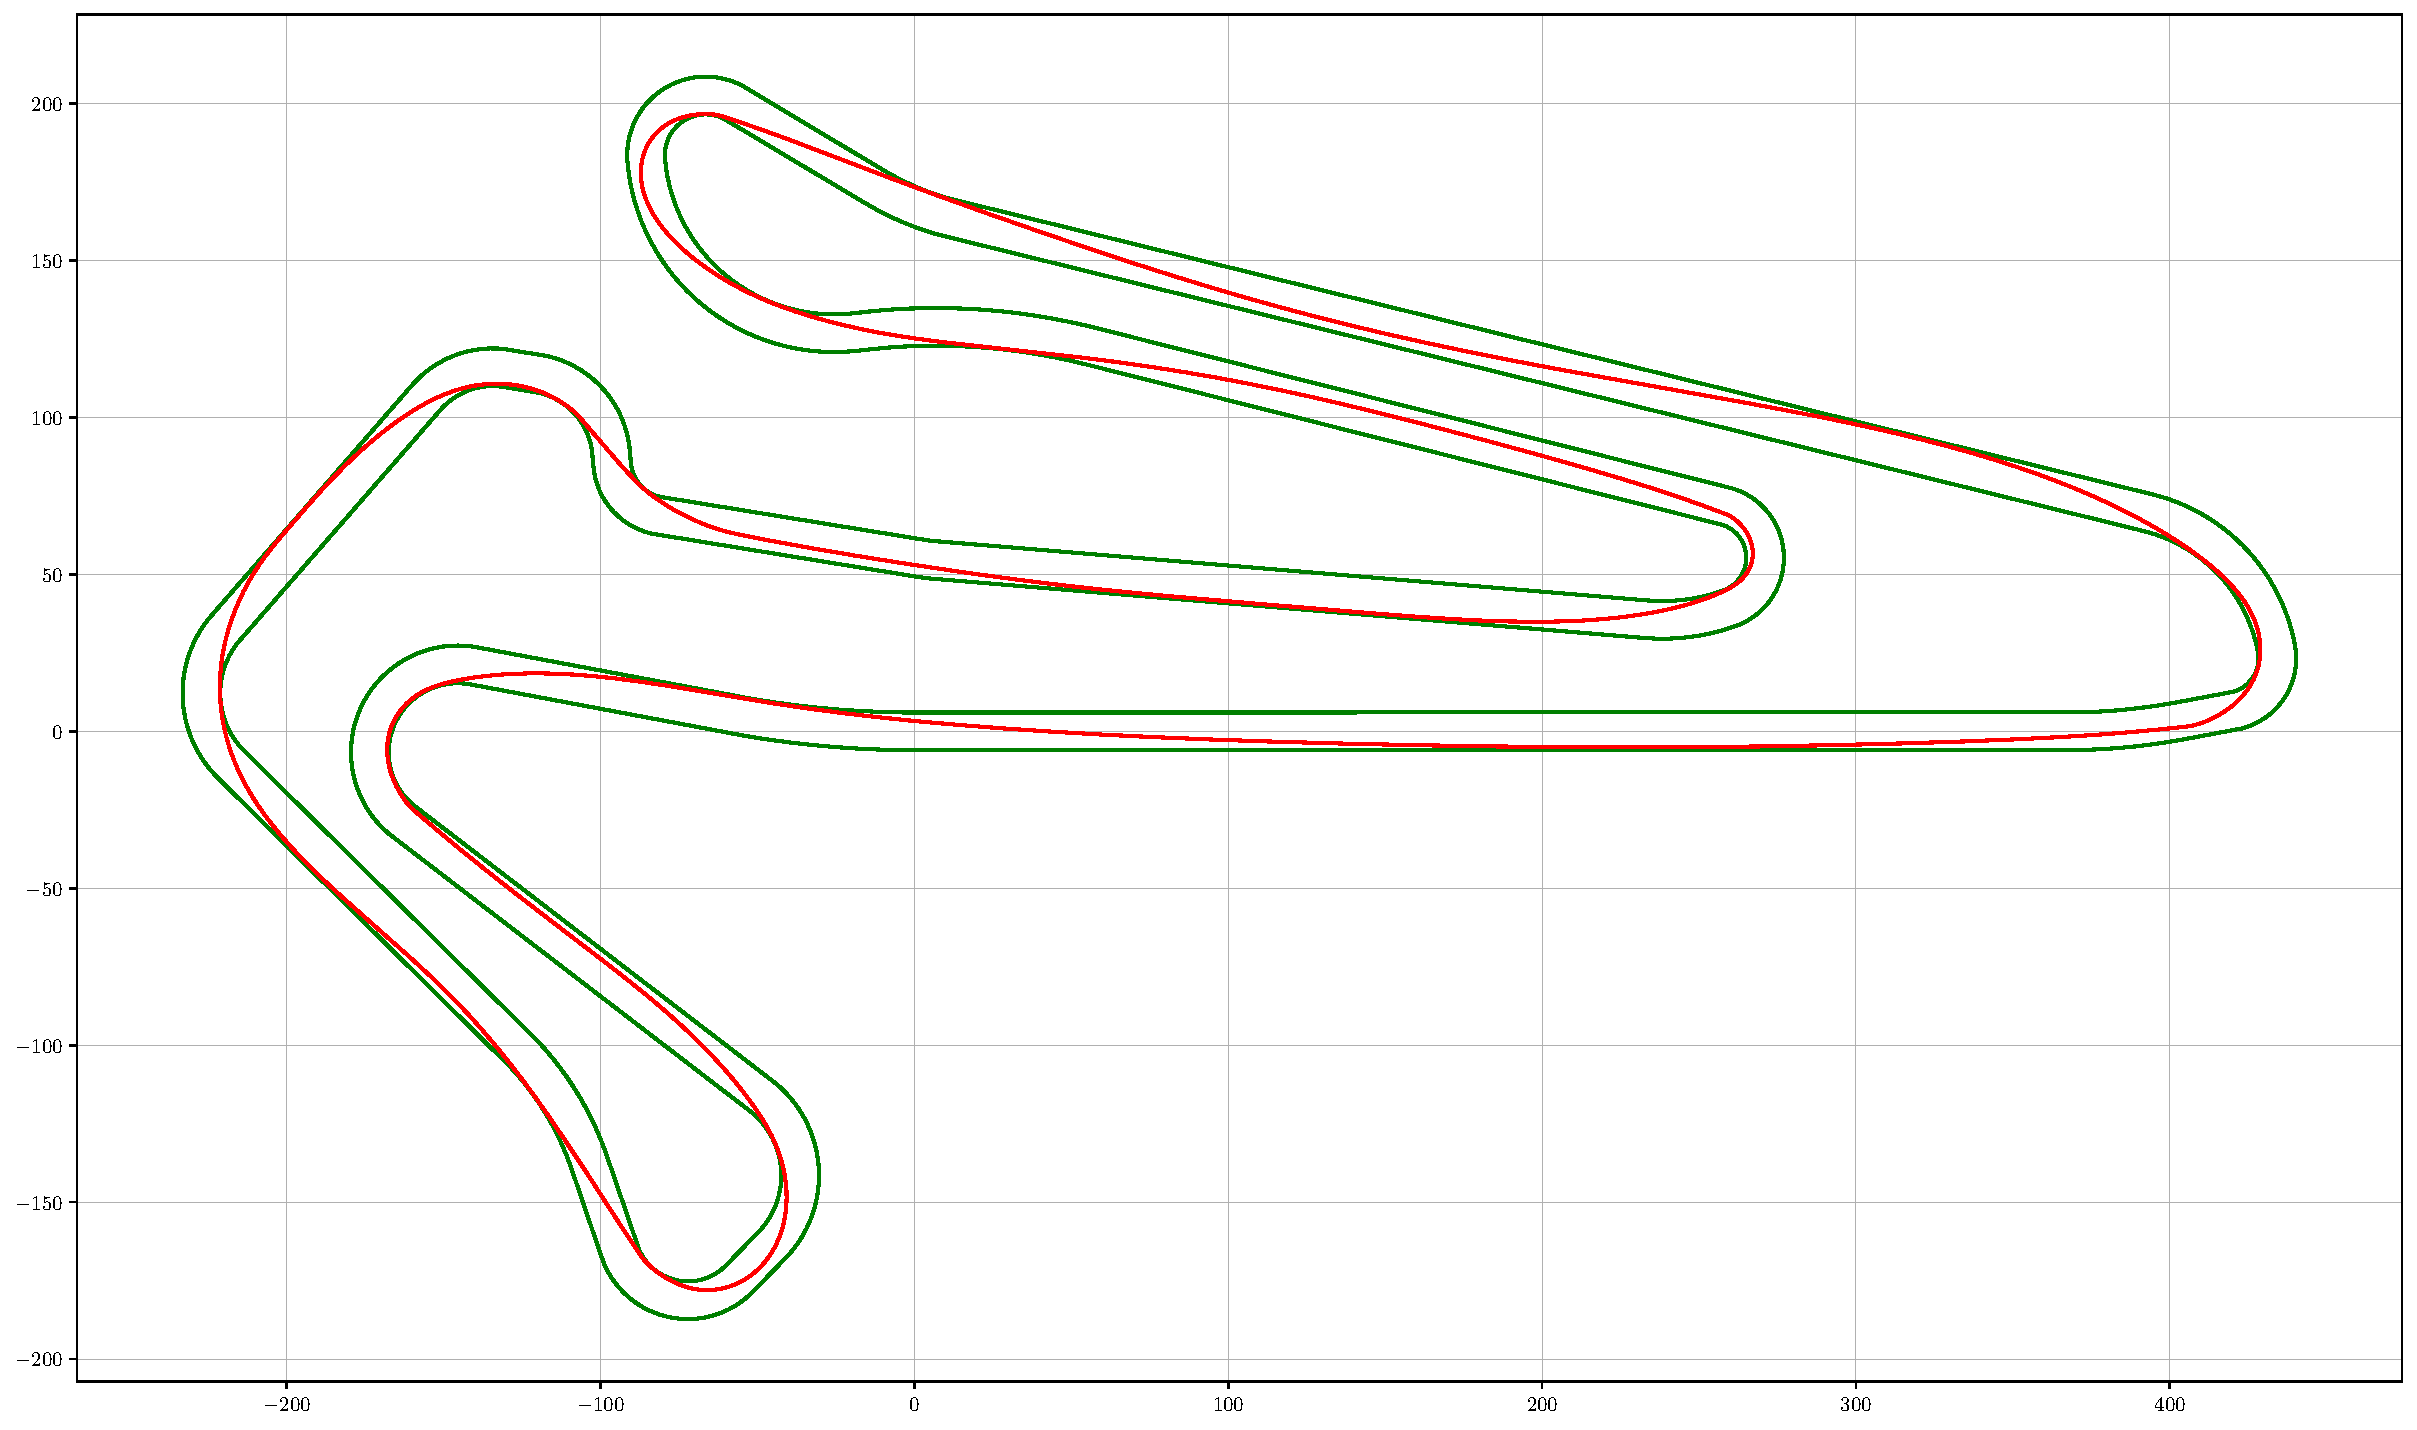
\includegraphics[angle=90,origin=c,height=1\linewidth]{Circuit/Track_P_SCell.pdf}
    \caption{Trajectory}
    \label{fig:TrajSCE}
\end{figure}
%
\clearpage
%
\section{Torque Control Adherence Ellipse Constraint}
%
\begin{figure}[!h]
    \centering
    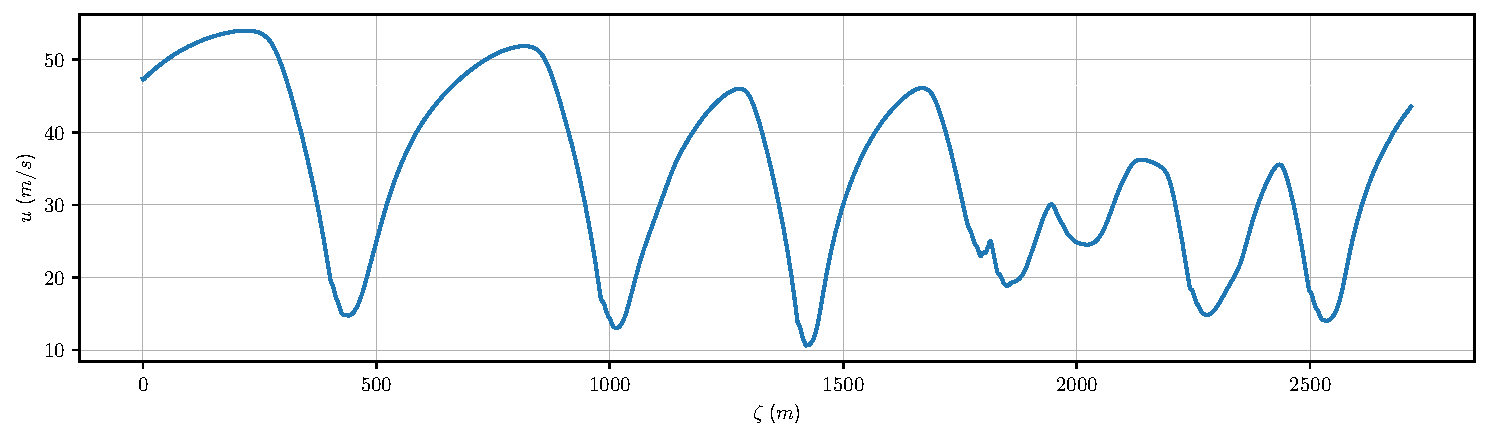
\includegraphics[width=\linewidth]{Circuit/u_P_TCell.pdf}
    \caption{Longitudinal speed}
    \label{fig:uTCE}
\end{figure}
%
\begin{figure}[!h]
    \centering
    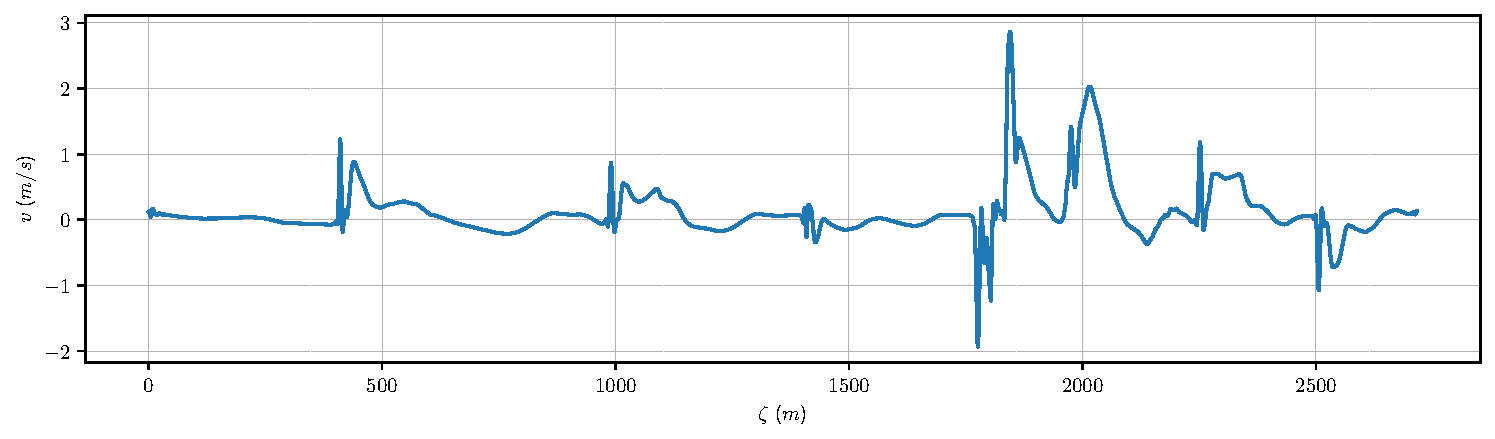
\includegraphics[width=\linewidth]{Circuit/v_P_TCell.pdf}
    \caption{Lateral speed}
    \label{fig:vTCE}
\end{figure}
%
\begin{figure}[!h]
    \centering
    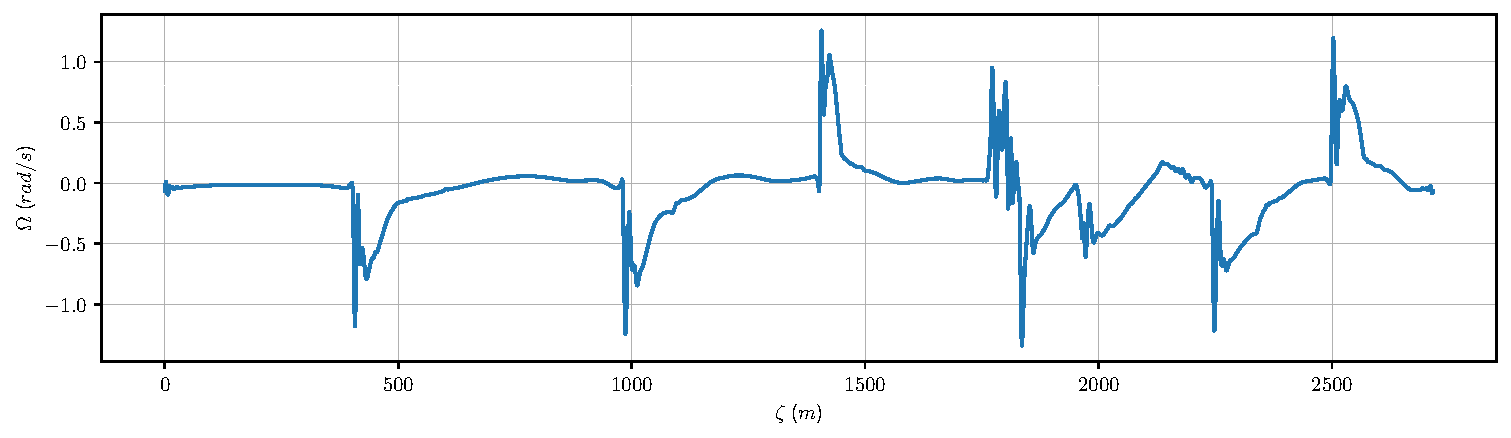
\includegraphics[width=\linewidth]{Circuit/Omega_P_TCell.pdf}
    \caption{Yaw rate}
    \label{fig:OmegaTCE}
\end{figure}
%
\begin{figure}[!h]
    \centering
    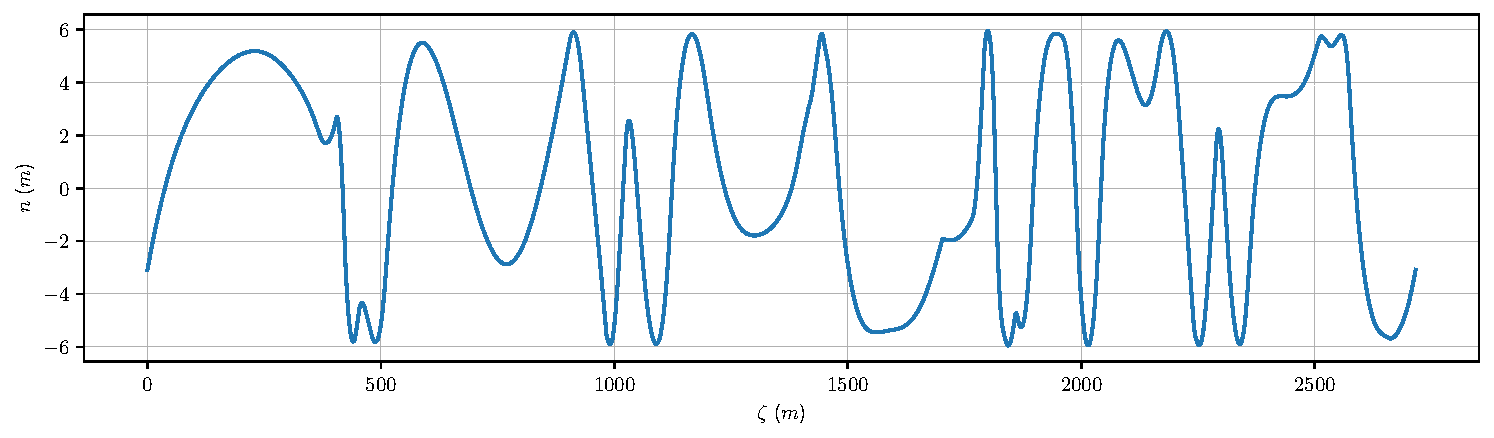
\includegraphics[width=\linewidth]{Circuit/n_P_TCell.pdf}
    \caption{Centreline deviation}
    \label{fig:nTCE}
\end{figure}
%
\begin{figure}[!h]
    \centering
    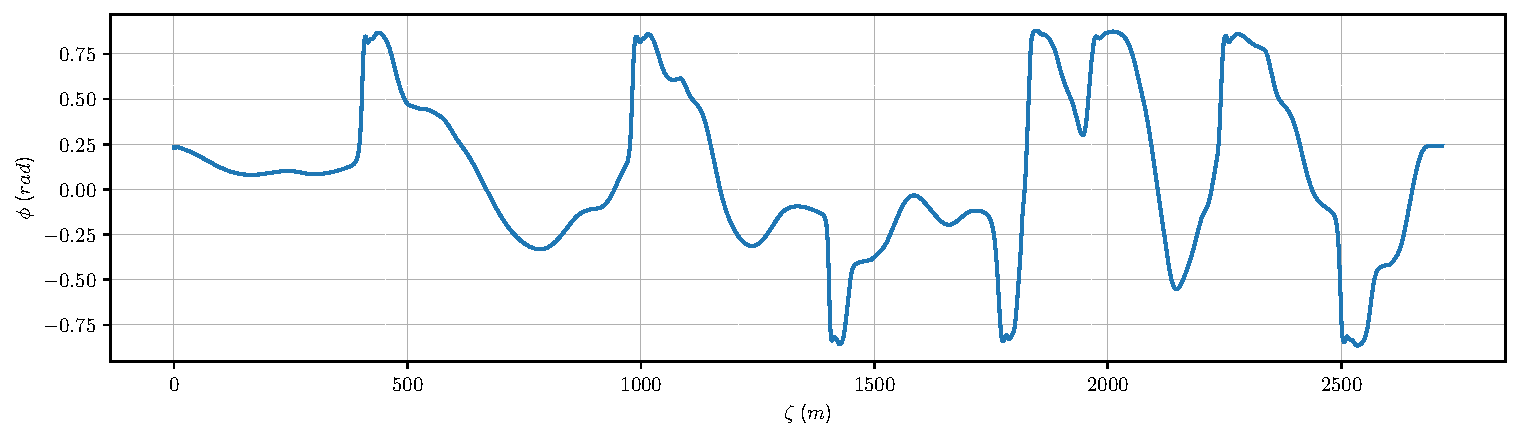
\includegraphics[width=\linewidth]{Circuit/phi_P_TCell.pdf}
    \caption{Roll angle}
    \label{fig:phiTCE}
\end{figure}
%
\begin{figure}[!h]
    \centering
    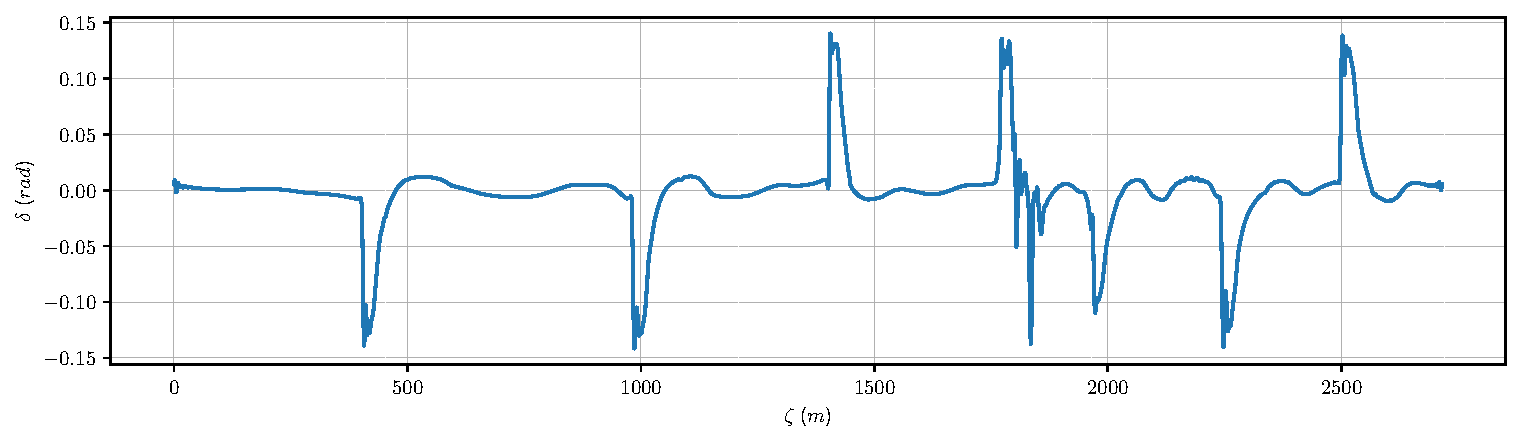
\includegraphics[width=\linewidth]{Circuit/delta_P_TCell.pdf}
    \caption{Steer angle}
    \label{fig:deltaTCE}
\end{figure}
%
\begin{figure}[!h]
    \centering
    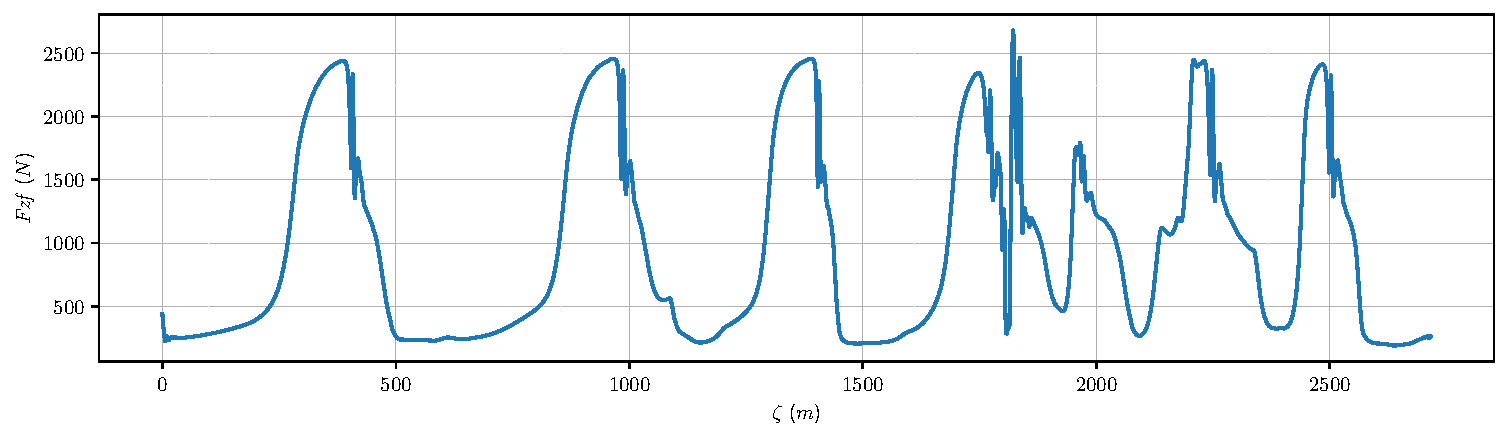
\includegraphics[width=\linewidth]{Circuit/Fzf_P_TCell.pdf}
    \caption{Vertical load front}
    \label{fig:FZFTCE}
\end{figure}
%
\begin{figure}[!h]
    \centering
    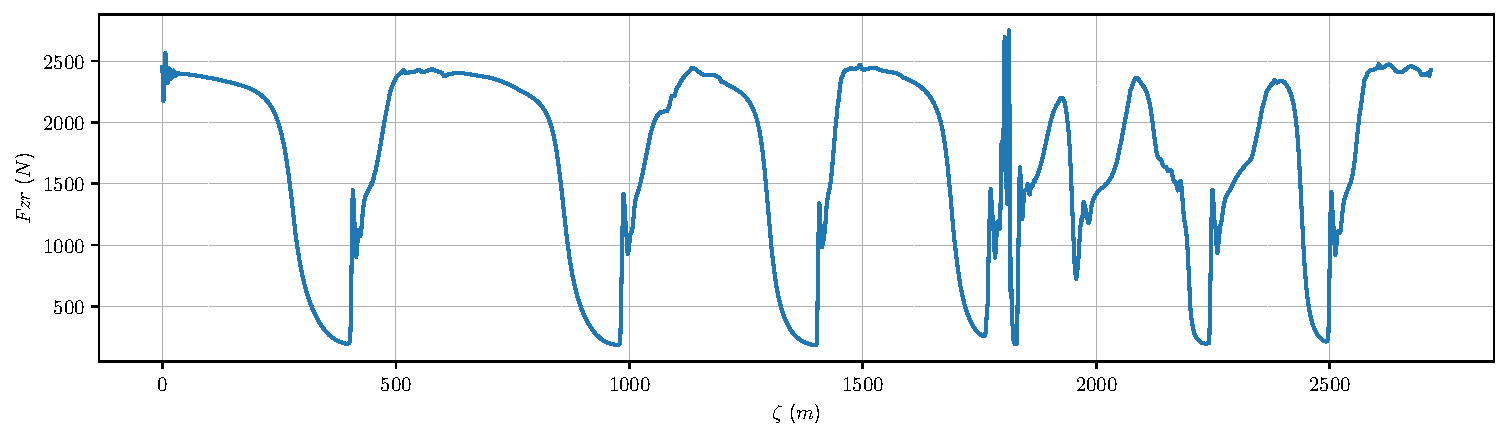
\includegraphics[width=\linewidth]{Circuit/Fzr_P_TCell.pdf}
    \caption{Vertical load rear}
    \label{fig:FZFTCE}
\end{figure}
%
\begin{figure}[!h]
    \begin{subfigure}{0.5\linewidth}
        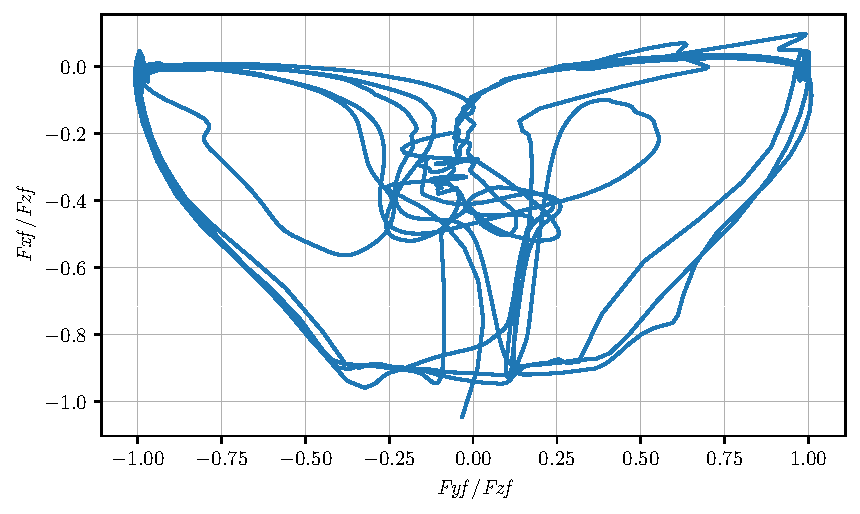
\includegraphics[width=\linewidth]{Circuit/EFront_P_TCell.pdf}
        \caption{Front}
        \label{fig:FETCE}
    \end{subfigure}%
    \begin{subfigure}{0.5\linewidth}
        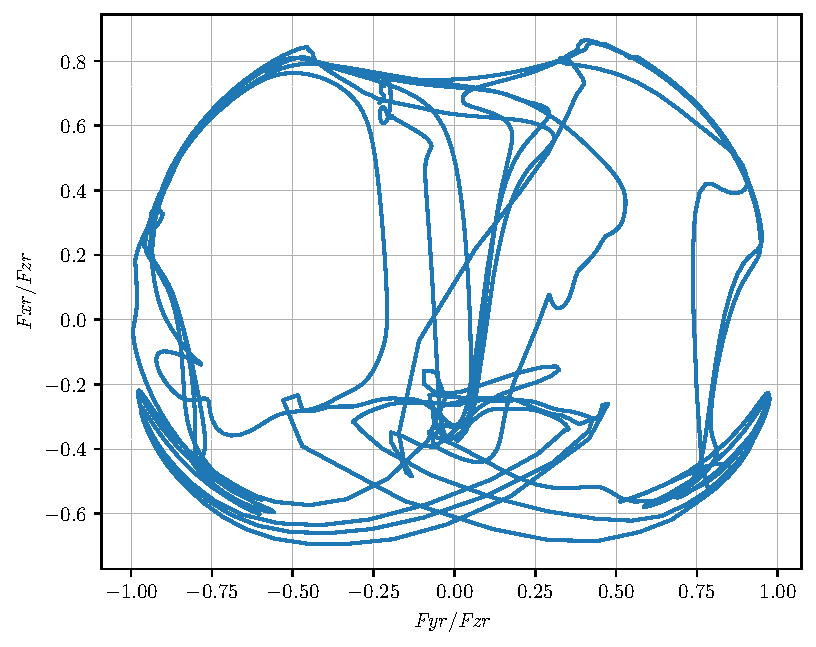
\includegraphics[width=\linewidth]{Circuit/ERear_P_TCell.pdf}
        \caption{Rear}
        \label{fig:RETCE}
    \end{subfigure}
    \caption{Ellipse of adherence}
\end{figure}
%
%
\begin{figure}[!h]
    \centering
    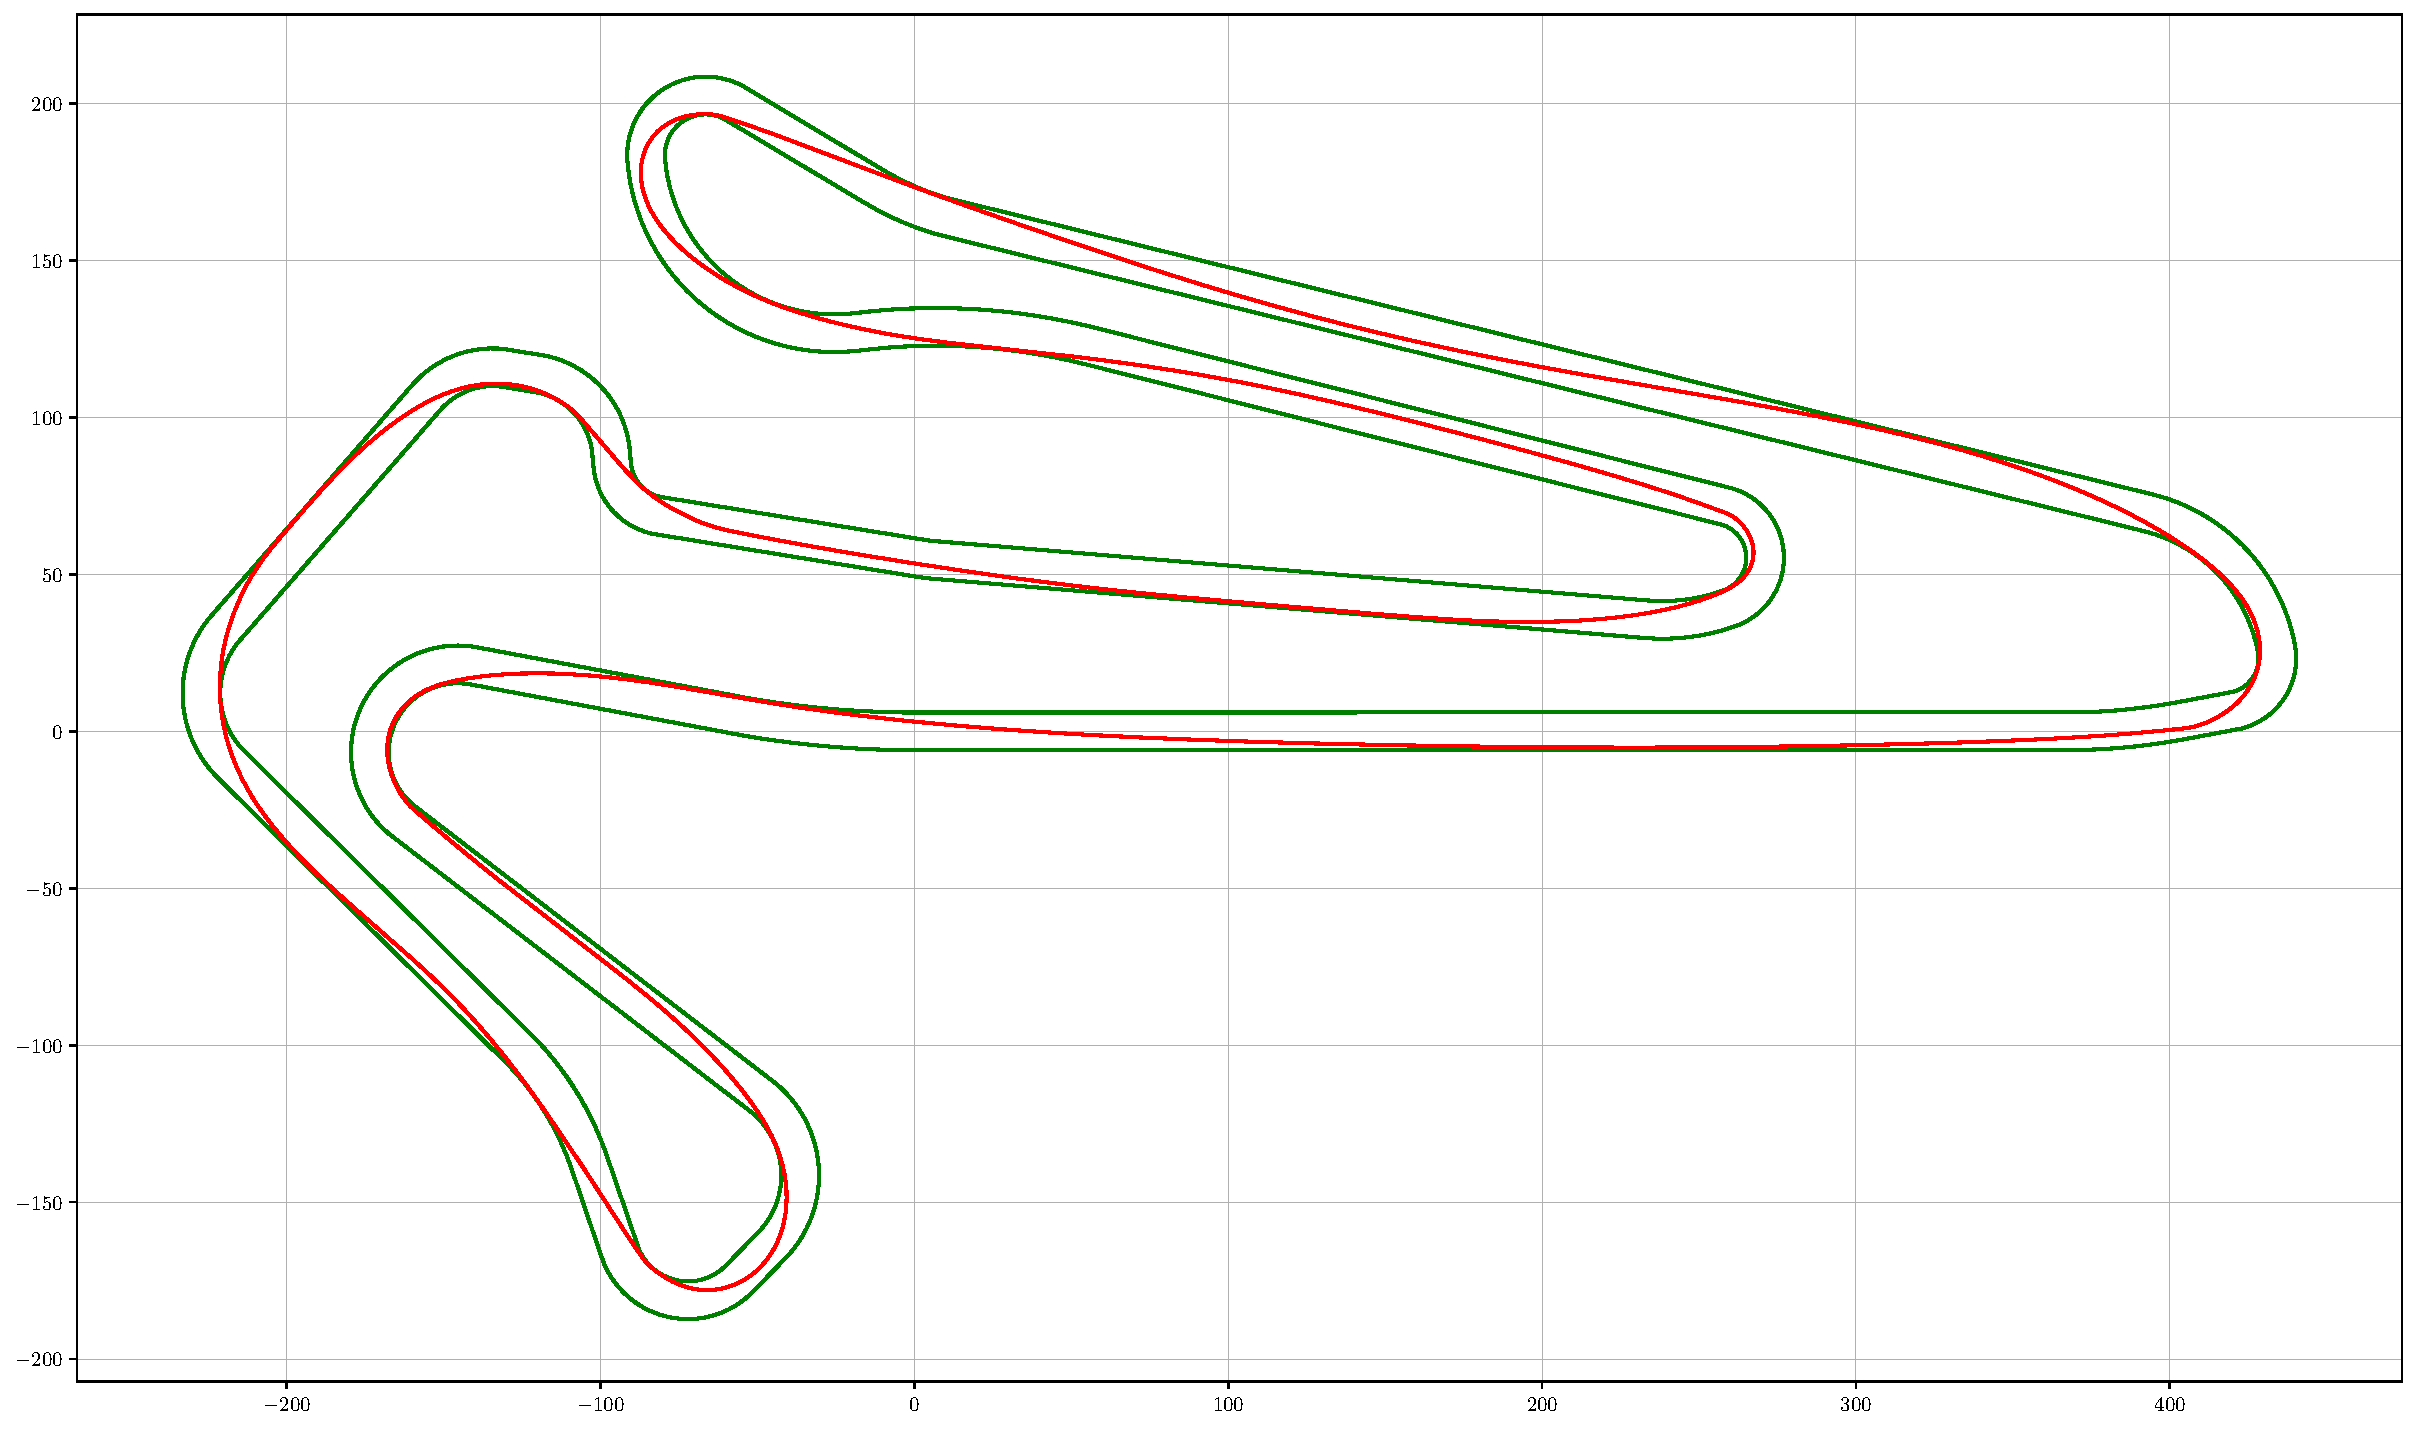
\includegraphics[angle=90,origin=c,height=1\linewidth]{Circuit/Track_P_TCell.pdf}
    \caption{Trajectory}
    \label{fig:TrajTCE}
\end{figure}
%
\clearpage
%
\section{Slip Control Combined Tyre Model}
%
\begin{figure}[!h]
    \centering
    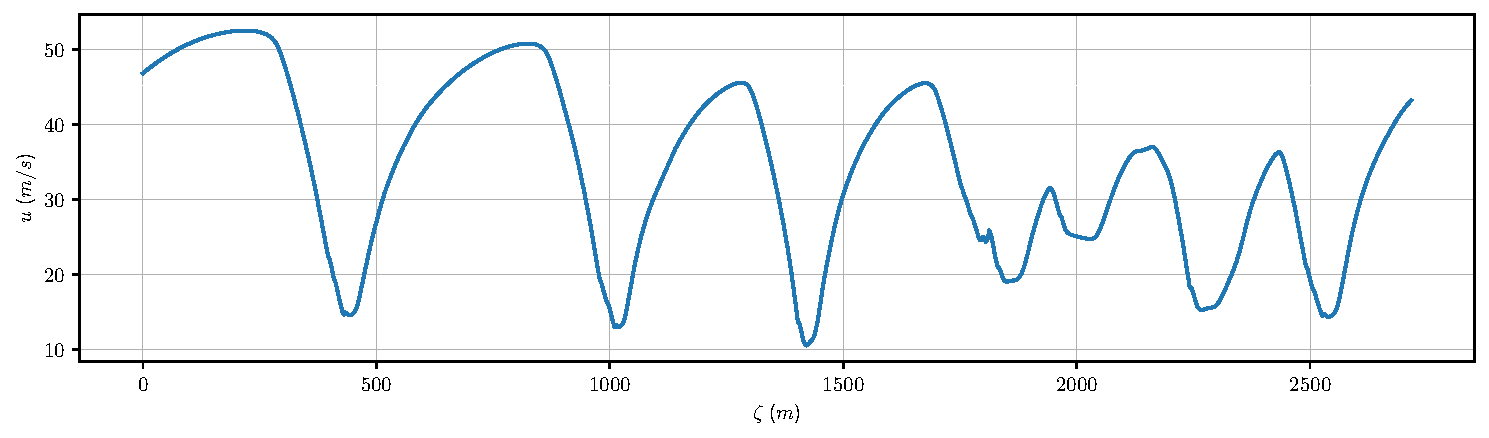
\includegraphics[width=\linewidth]{Circuit/u_P_SCcomb.pdf}
    \caption{Longitudinal speed}
    \label{fig:uSCC}
\end{figure}
%
\begin{figure}[!h]
    \centering
    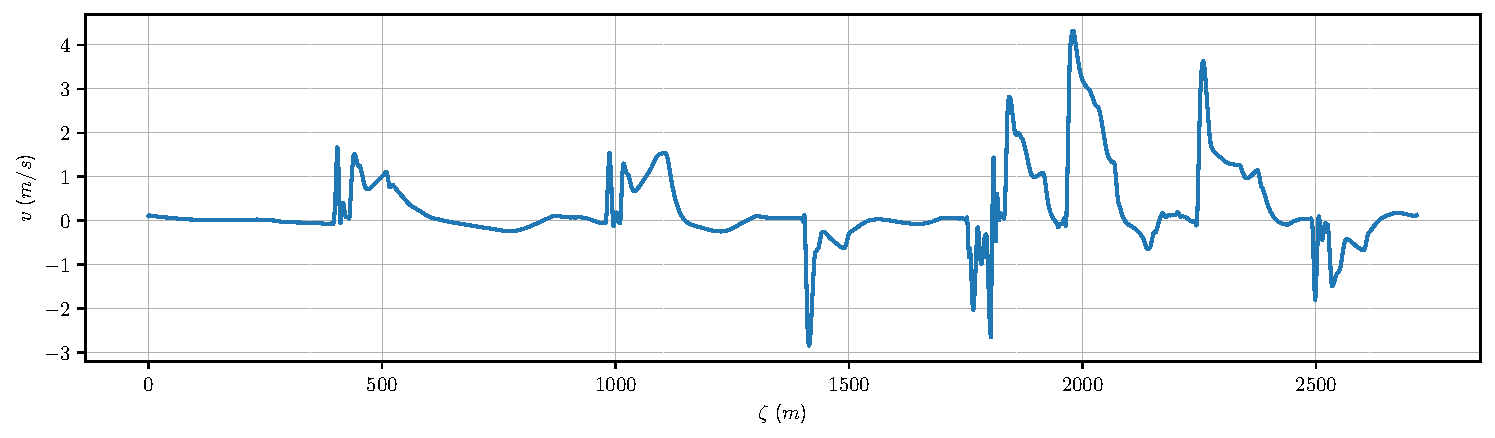
\includegraphics[width=\linewidth]{Circuit/v_P_SCcomb.pdf}
    \caption{Lateral speed}
    \label{fig:vSCC}
\end{figure}
%
\begin{figure}[!h]
    \centering
    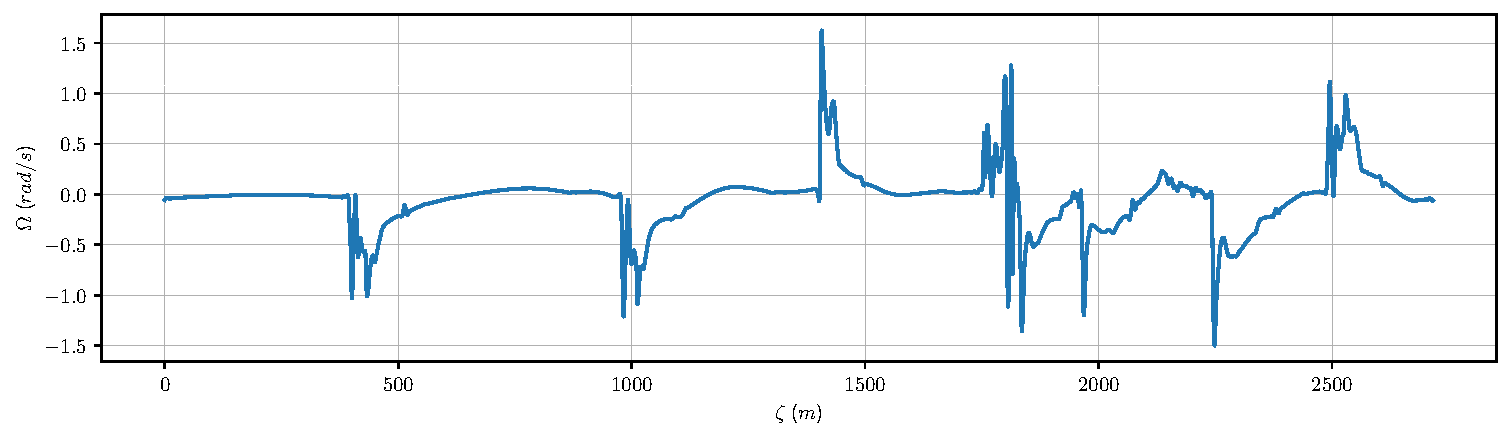
\includegraphics[width=\linewidth]{Circuit/Omega_P_SCcomb.pdf}
    \caption{Yaw rate}
    \label{fig:OmegaSCC}
\end{figure}
%
\begin{figure}[!h]
    \centering
    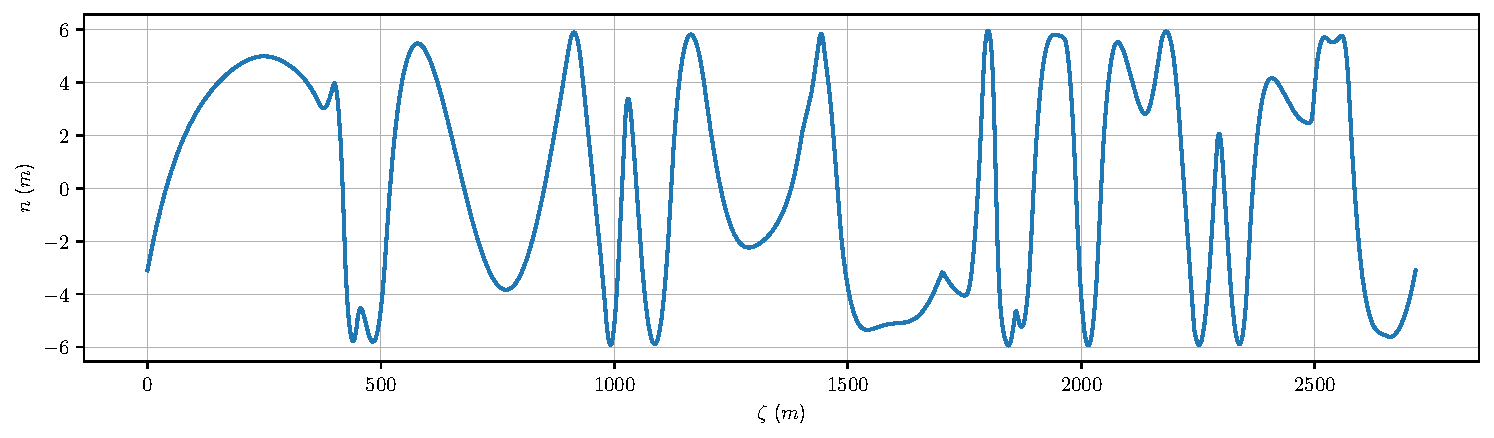
\includegraphics[width=\linewidth]{Circuit/n_P_SCcomb.pdf}
    \caption{Centreline deviation}
    \label{fig:nSCC}
\end{figure}
%
\begin{figure}[!h]
    \centering
    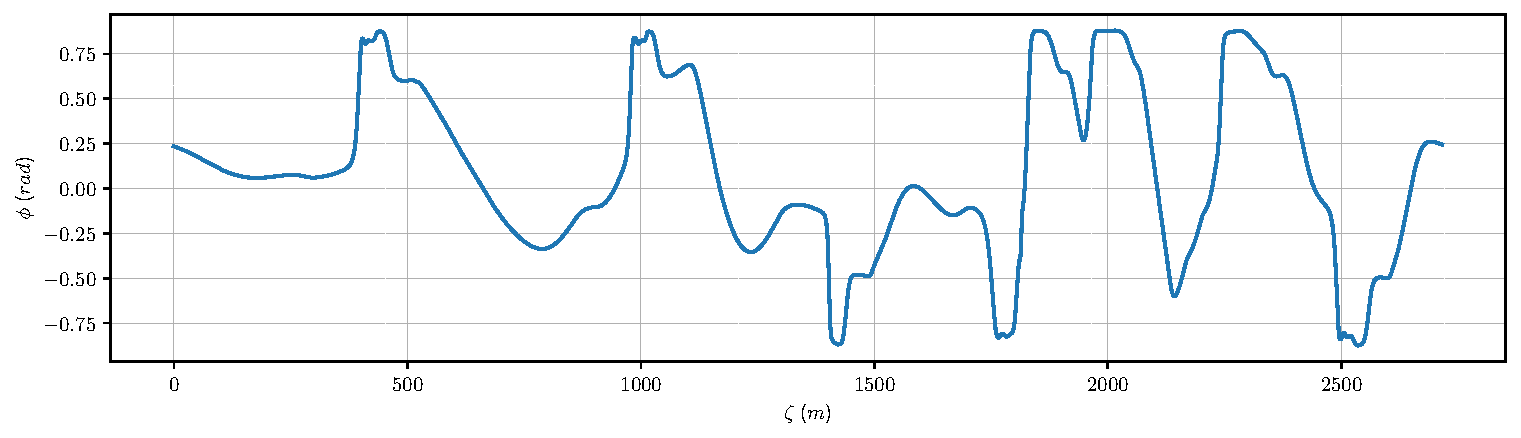
\includegraphics[width=\linewidth]{Circuit/phi_P_SCcomb.pdf}
    \caption{Roll angle}
    \label{fig:phiSCC}
\end{figure}
%
\begin{figure}[!h]
    \centering
    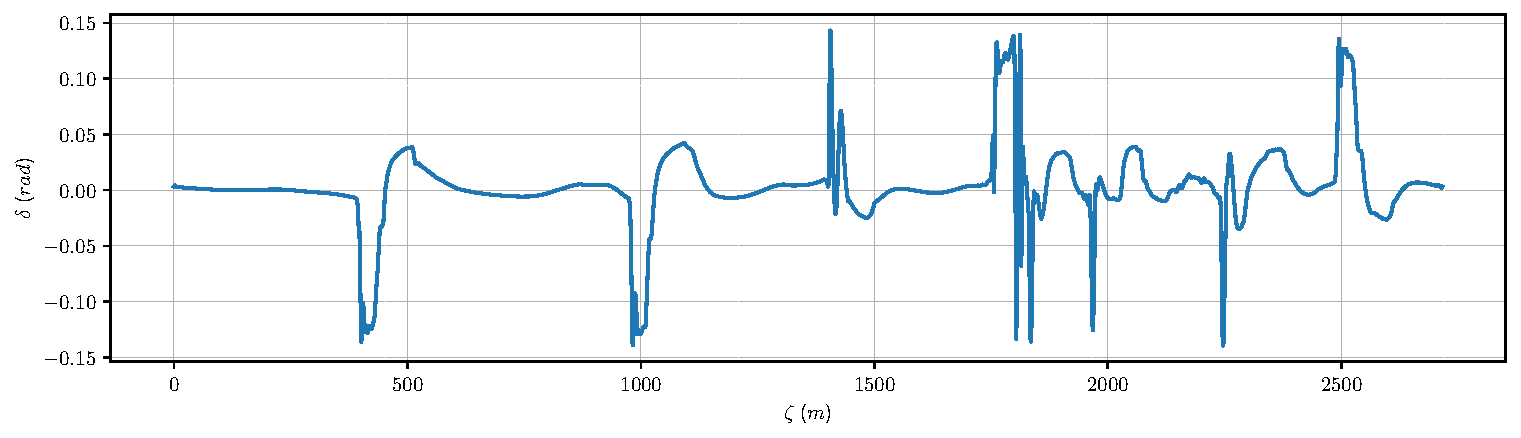
\includegraphics[width=\linewidth]{Circuit/delta_P_SCcomb.pdf}
    \caption{Steer angle}
    \label{fig:deltaSCC}
\end{figure}
%
\begin{figure}[!h]
    \centering
    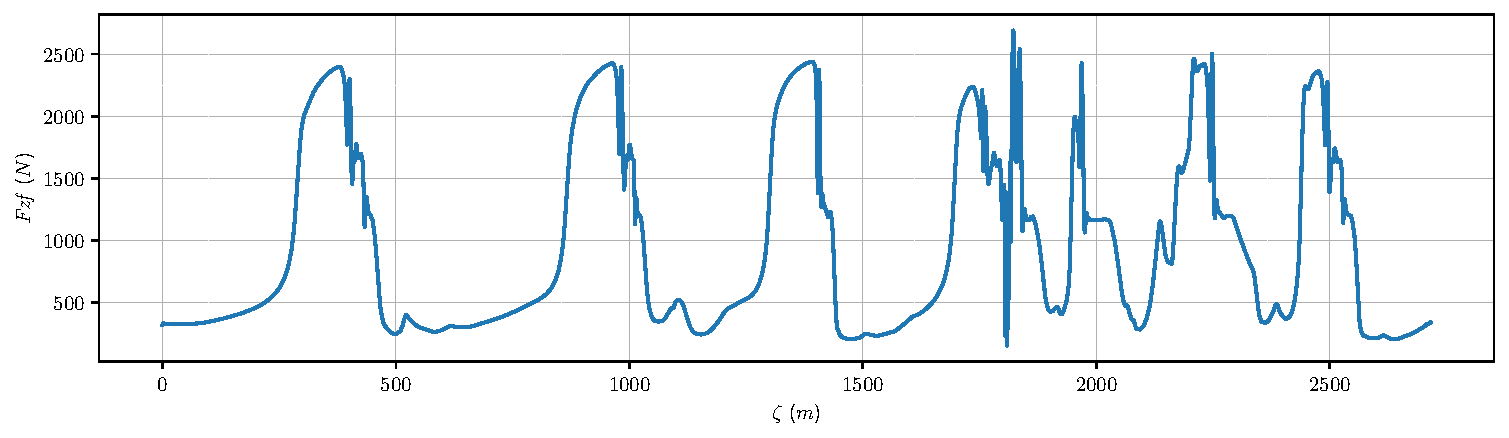
\includegraphics[width=\linewidth]{Circuit/Fzf_P_SCcomb.pdf}
    \caption{Vertical load front}
    \label{fig:FZFSCC}
\end{figure}
%
\begin{figure}[!h]
    \centering
    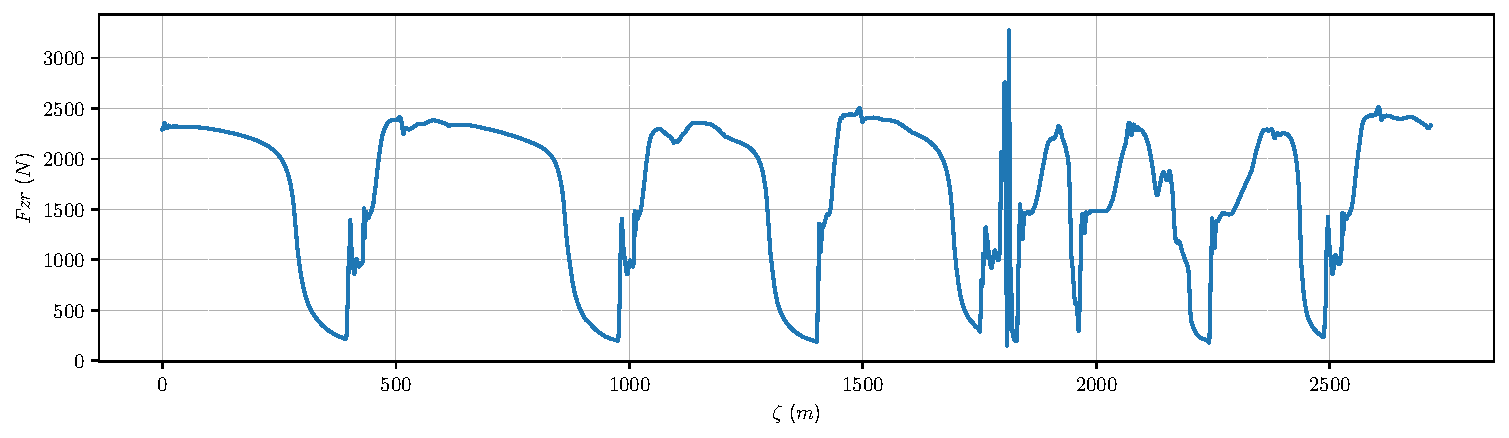
\includegraphics[width=\linewidth]{Circuit/Fzr_P_SCcomb.pdf}
    \caption{Vertical load rear}
    \label{fig:FZFSCC}
\end{figure}
%
\begin{figure}[!h]
    \begin{subfigure}{0.5\linewidth}
        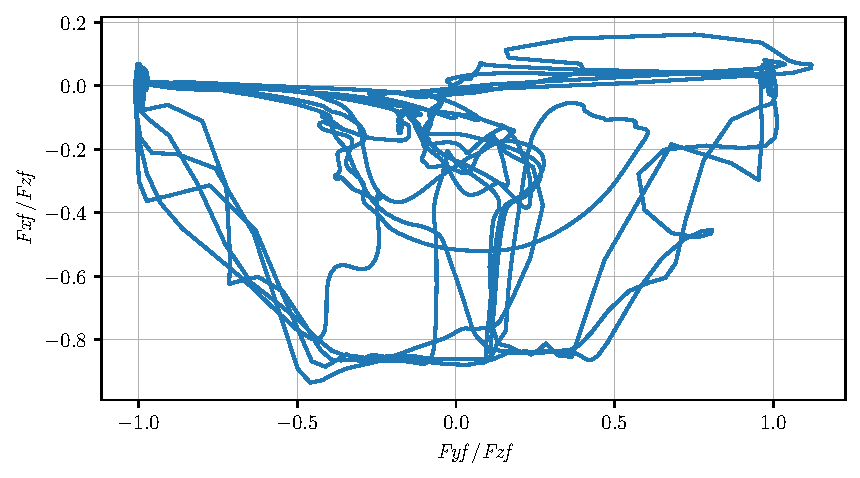
\includegraphics[width=\linewidth]{Circuit/EFront_P_SCcomb.pdf}
        \caption{Front}
        \label{fig:FESCC}
    \end{subfigure}%
    \begin{subfigure}{0.5\linewidth}
        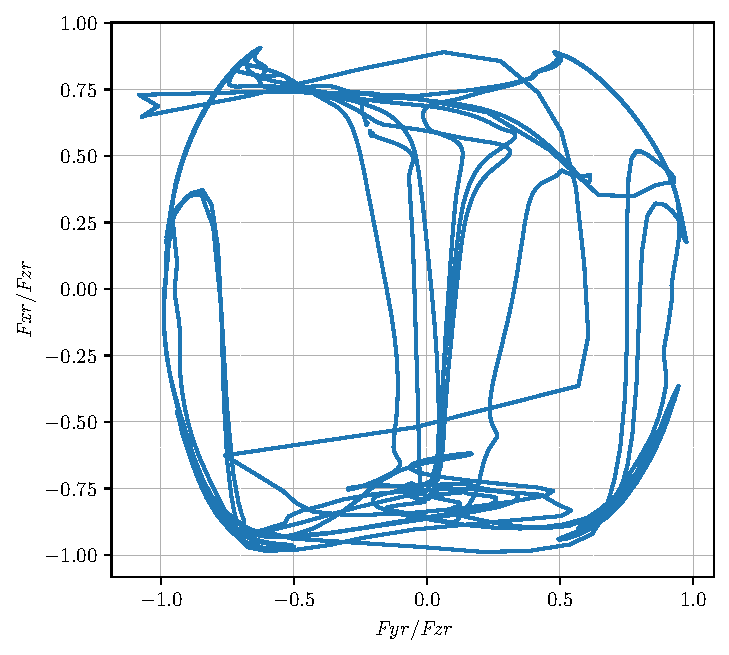
\includegraphics[width=\linewidth]{Circuit/ERear_P_SCcomb.pdf}
        \caption{Rear}
        \label{fig:RESCC}
    \end{subfigure}
    \caption{Ellipse of adherence}
\end{figure}
%
%
\begin{figure}[!h]
    \centering
    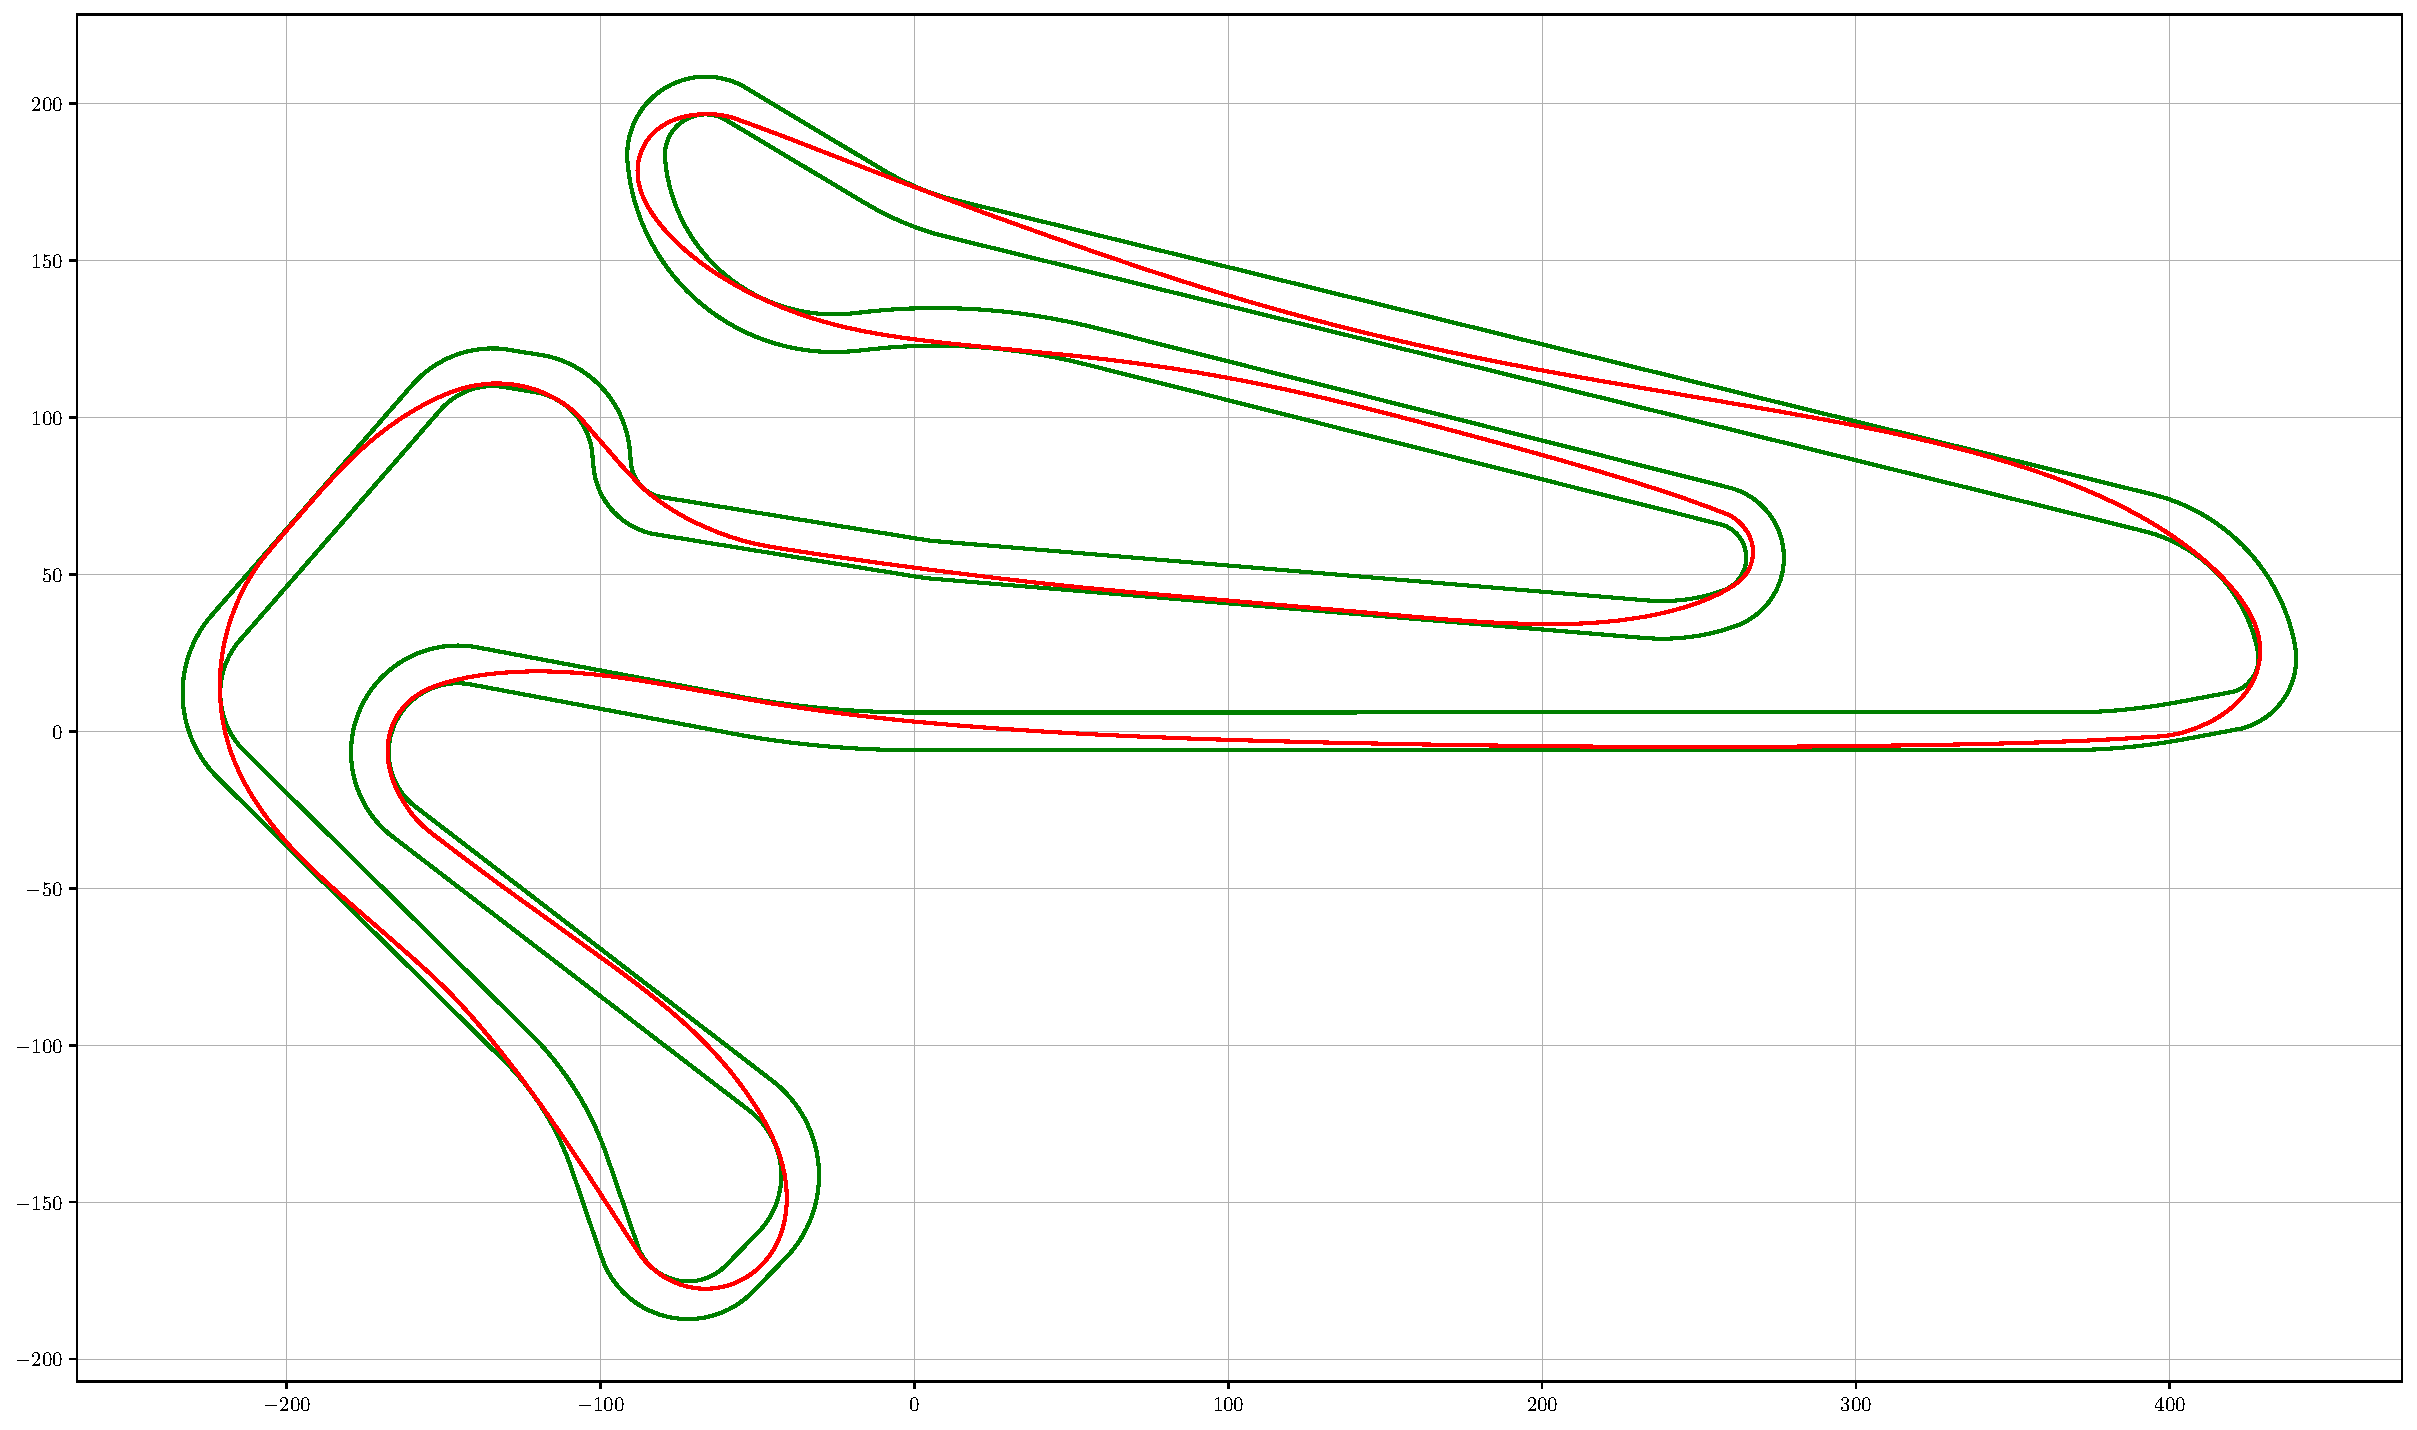
\includegraphics[angle=90,origin=c,height=1\linewidth]{Circuit/Track_P_SCcomb.pdf}
    \caption{Trajectory}
    \label{fig:TrajSCC}
\end{figure}
%
\clearpage
%
\section{Torque Control Combined Tyre Model}
%
\begin{figure}[!h]
    \centering
    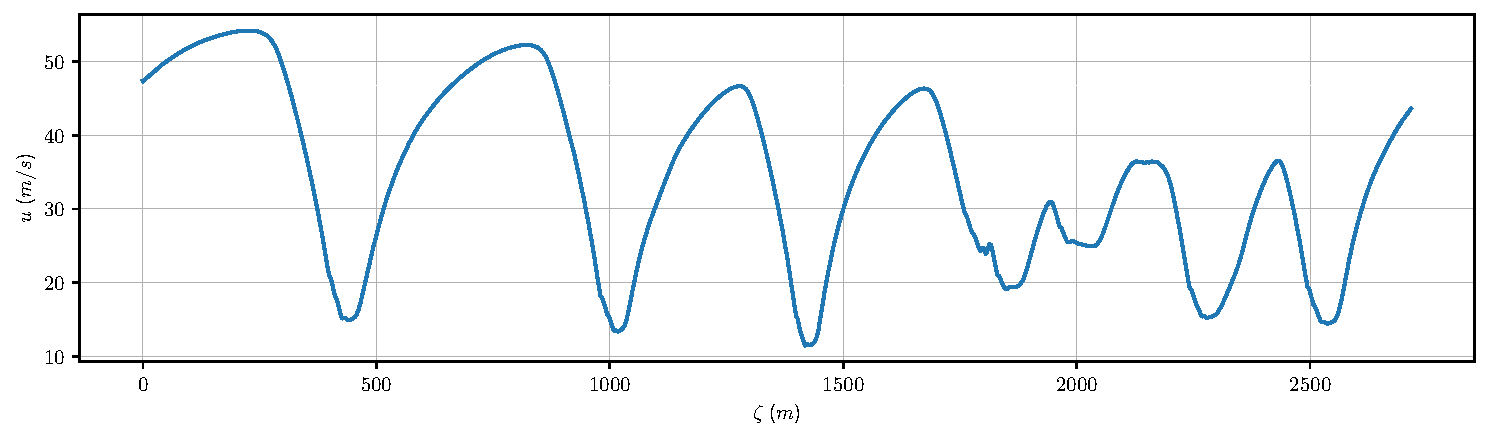
\includegraphics[width=\linewidth]{Circuit/u_P_TCcomb.pdf}
    \caption{Longitudinal speed}
    \label{fig:uTCC}
\end{figure}
%
\begin{figure}[!h]
    \centering
    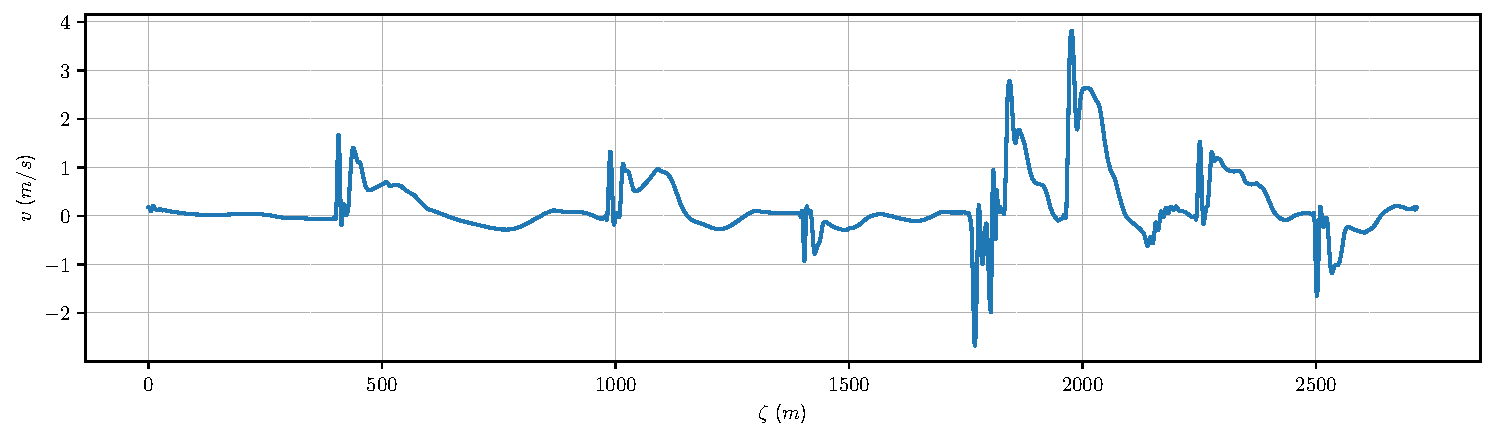
\includegraphics[width=\linewidth]{Circuit/v_P_TCcomb.pdf}
    \caption{Lateral speed}
    \label{fig:vTCC}
\end{figure}
%
\begin{figure}[!h]
    \centering
    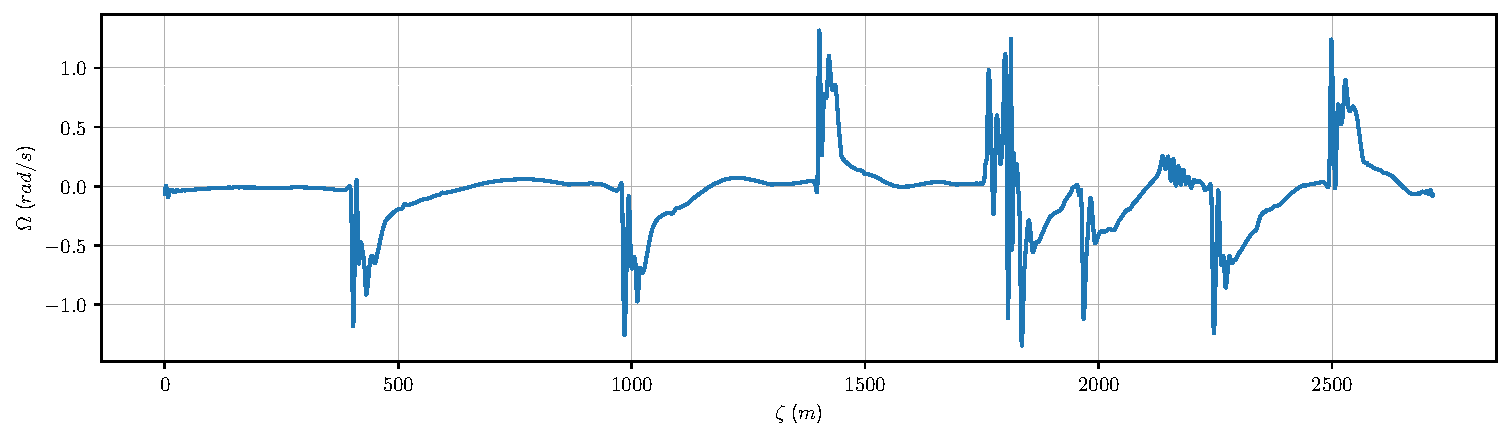
\includegraphics[width=\linewidth]{Circuit/Omega_P_TCcomb.pdf}
    \caption{Yaw rate}
    \label{fig:OmegaTCC}
\end{figure}
%
\begin{figure}[!h]
    \centering
    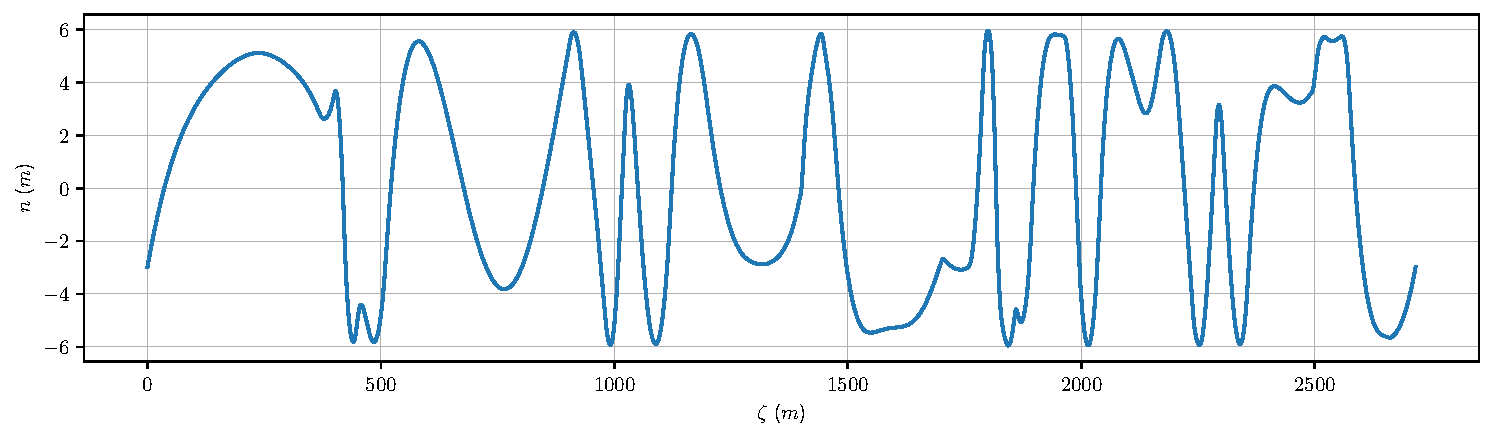
\includegraphics[width=\linewidth]{Circuit/n_P_TCcomb.pdf}
    \caption{Centreline deviation}
    \label{fig:nTCC}
\end{figure}
%
\begin{figure}[!h]
    \centering
    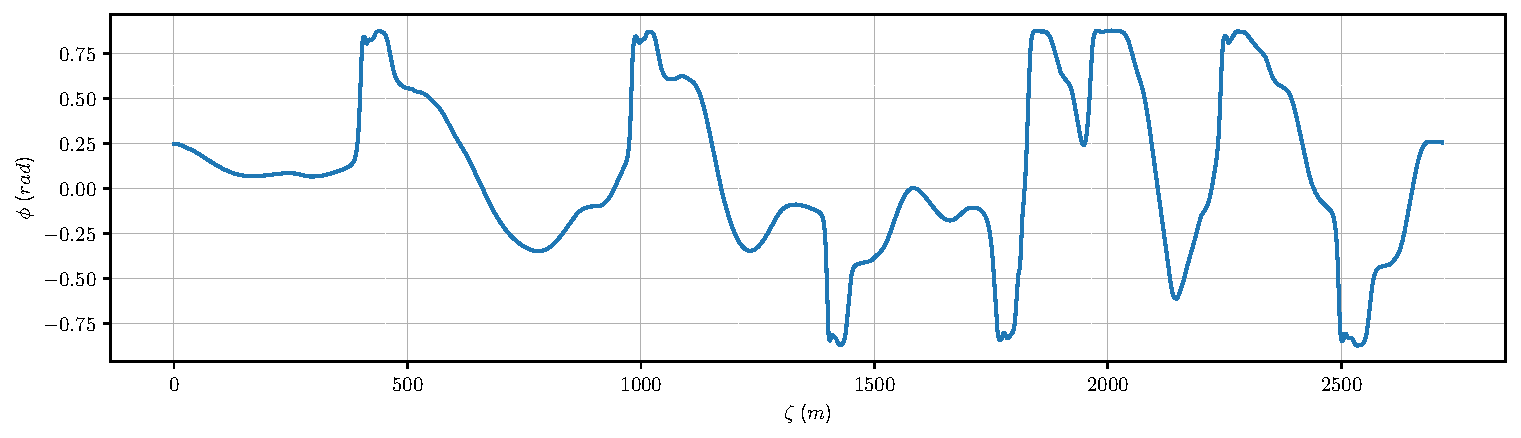
\includegraphics[width=\linewidth]{Circuit/phi_P_TCcomb.pdf}
    \caption{Roll angle}
    \label{fig:phiTCC}
\end{figure}
%
\begin{figure}[!h]
    \centering
    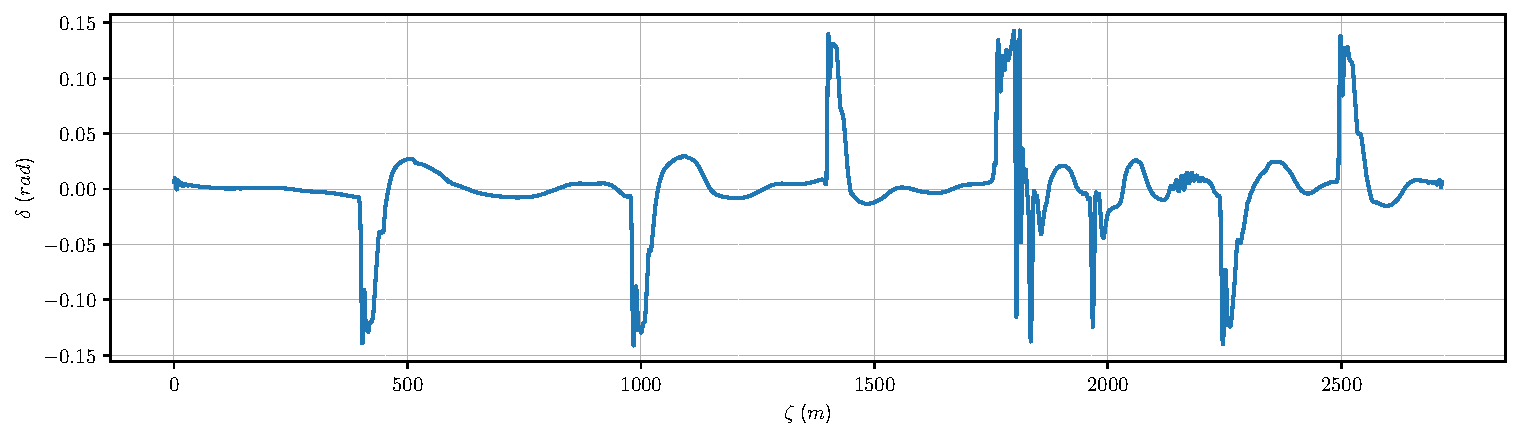
\includegraphics[width=\linewidth]{Circuit/delta_P_TCcomb.pdf}
    \caption{Steer angle}
    \label{fig:deltaTCC}
\end{figure}
%
\begin{figure}[!h]
    \centering
    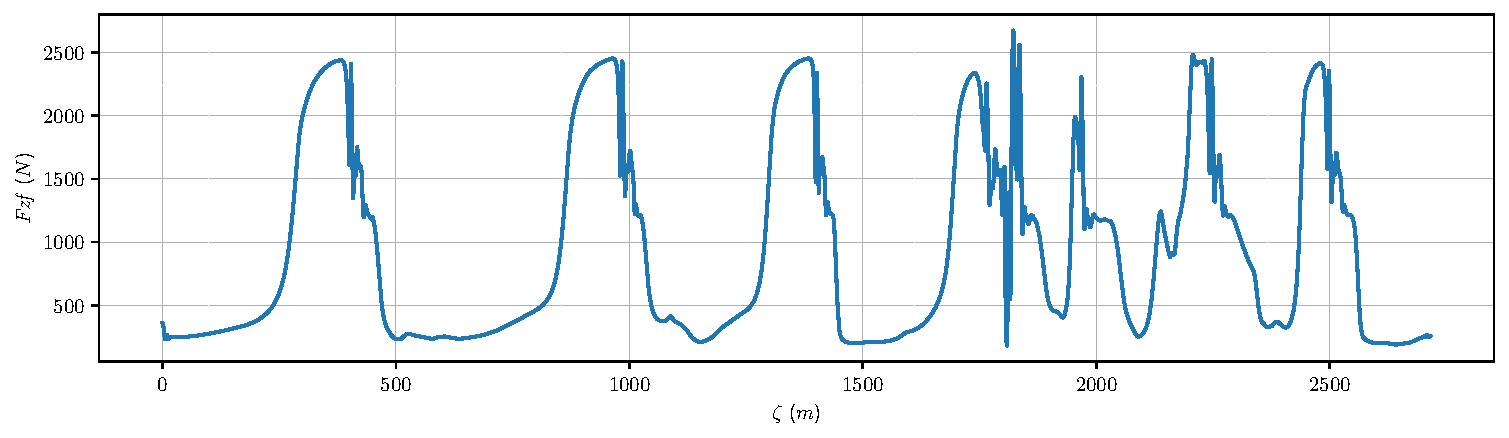
\includegraphics[width=\linewidth]{Circuit/Fzf_P_TCcomb.pdf}
    \caption{Vertical load front}
    \label{fig:FZFTCC}
\end{figure}
%
\begin{figure}[!h]
    \centering
    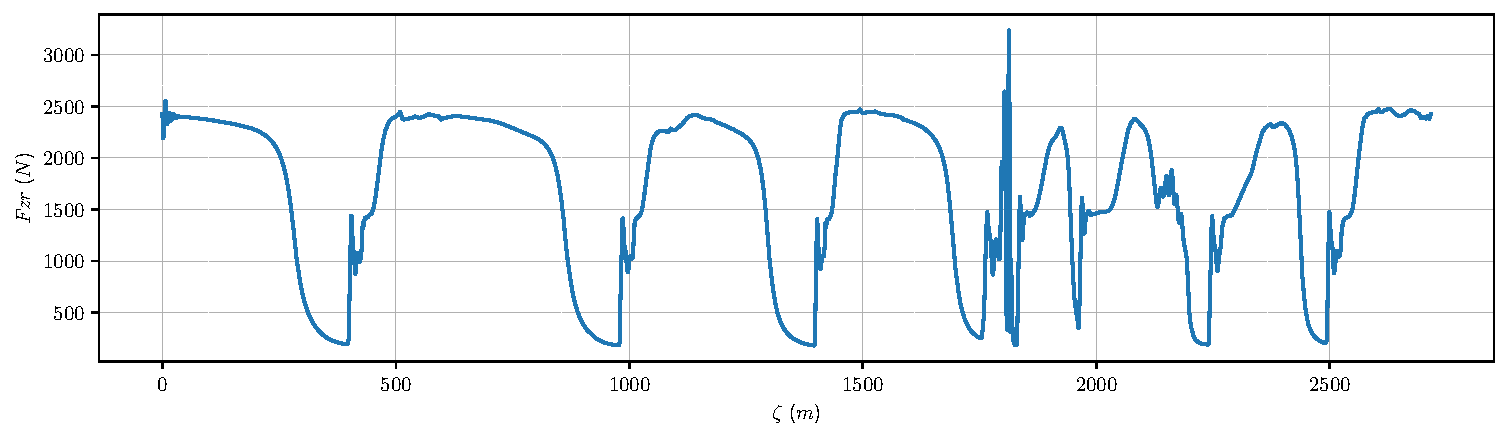
\includegraphics[width=\linewidth]{Circuit/Fzr_P_TCcomb.pdf}
    \caption{Vertical load rear}
    \label{fig:FZFTCC}
\end{figure}
%
\begin{figure}[!h]
    \begin{subfigure}{0.5\linewidth}
        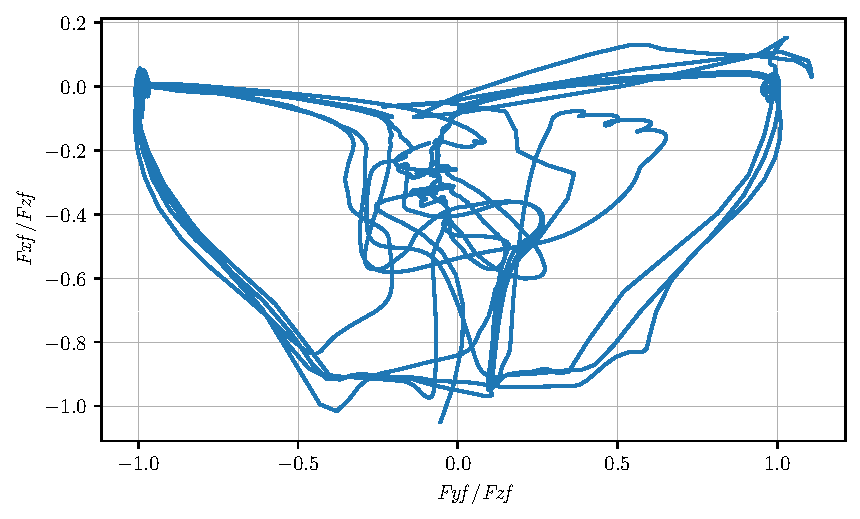
\includegraphics[width=\linewidth]{Circuit/EFront_P_TCcomb.pdf}
        \caption{Front}
        \label{fig:FETCC}
    \end{subfigure}%
    \begin{subfigure}{0.5\linewidth}
        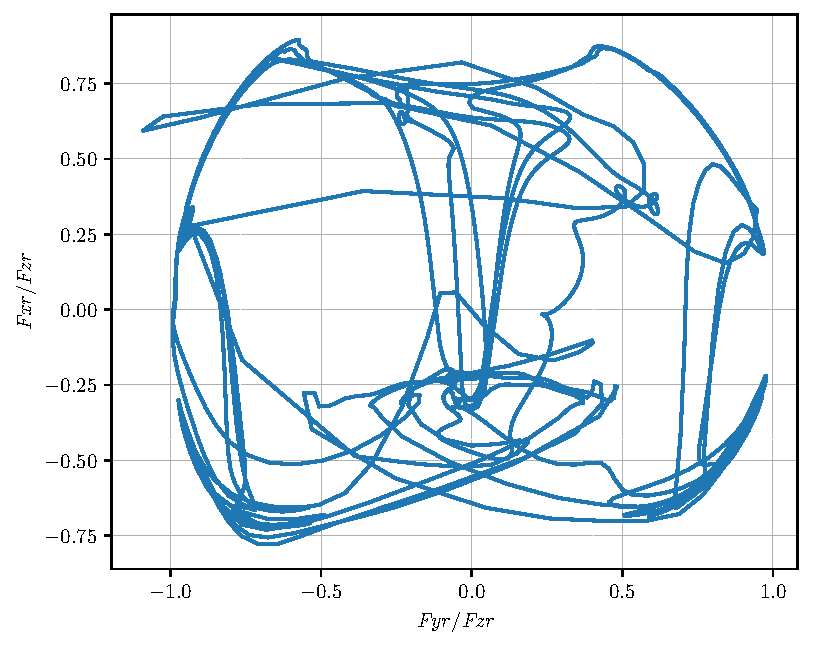
\includegraphics[width=\linewidth]{Circuit/ERear_P_TCcomb.pdf}
        \caption{Rear}
        \label{fig:RETCC}
    \end{subfigure}
    \caption{Ellipse of adherence}
\end{figure}
%
%
\begin{figure}[!h]
    \centering
    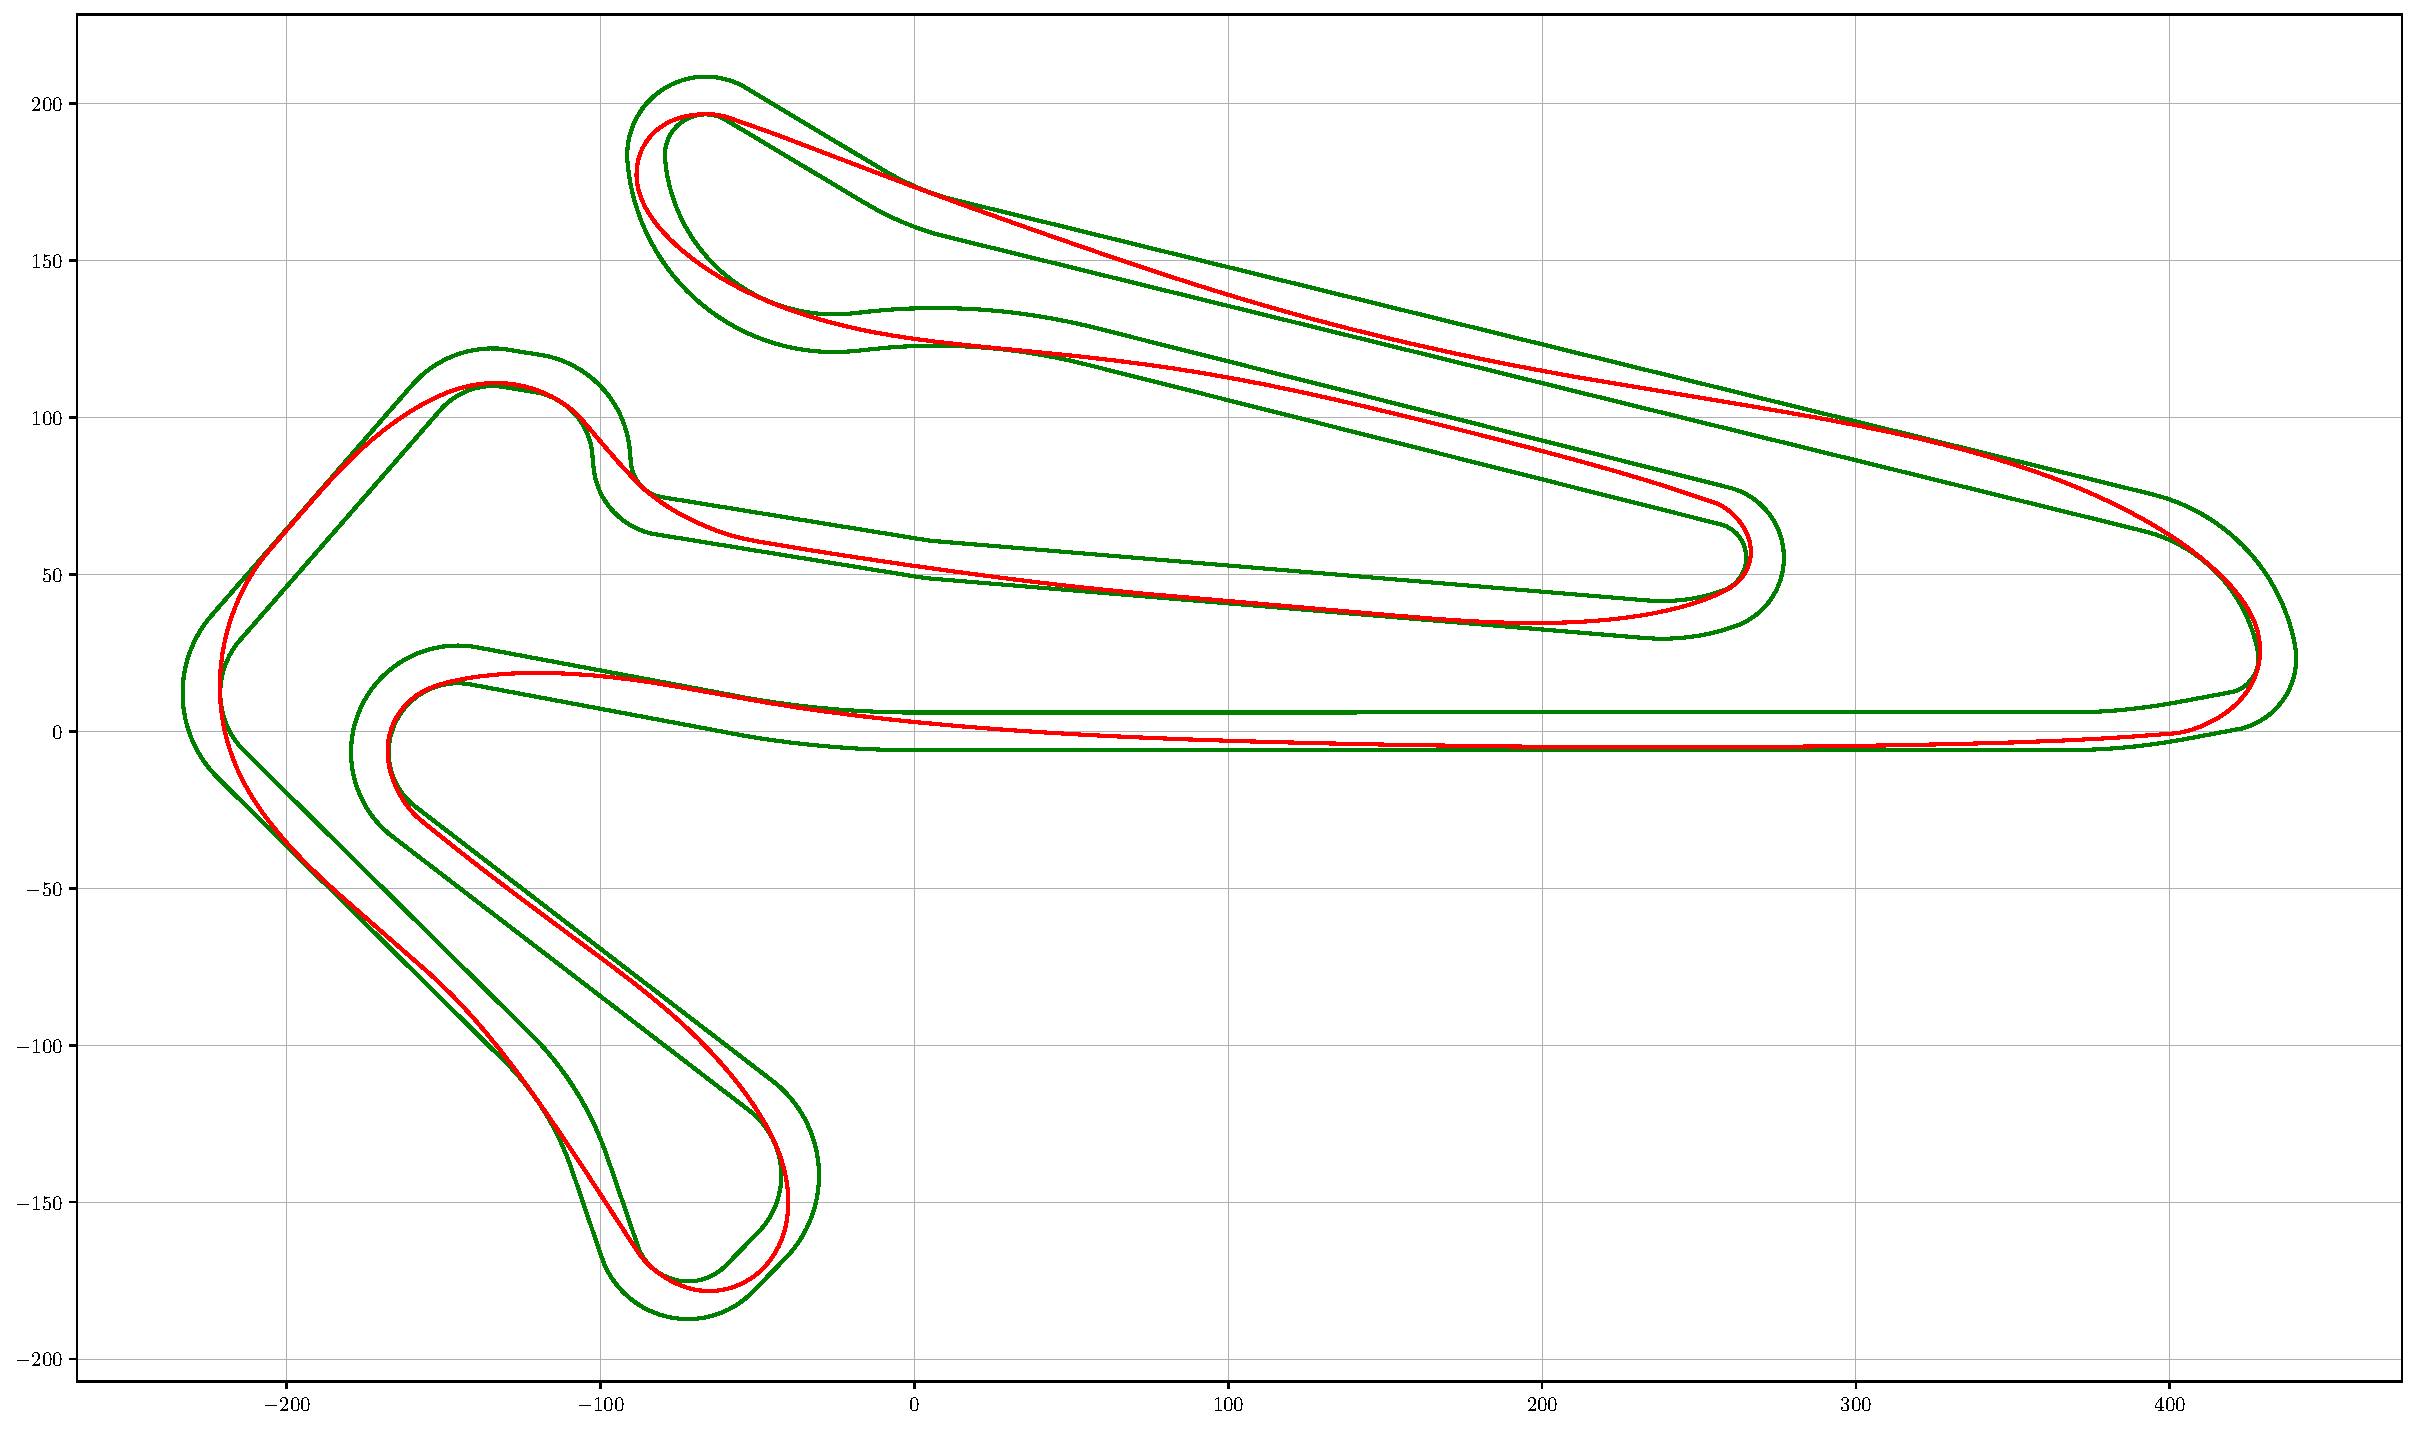
\includegraphics[angle=90,origin=c,height=1\linewidth]{Circuit/Track_P_TCcomb.pdf}
    \caption{Trajectory}
    \label{fig:TrajTCC}
\end{figure}
%
\clearpage
%